\documentclass[8pt]{beamer}

\newif\ifplacelogo % create a new conditional
\placelogotrue % set it to true

\usetheme{Warsaw}
\usecolortheme{rose}
\usepackage{multicol}
\usepackage{epstopdf}
\usepackage[italic]{hepnames}
\usepackage{tikz}
\usepackage{listings}
\usepackage{times}
\usepackage{amsmath}
\usepackage{verbatim}
\usepackage{hyperref}
\usepackage{bbding}
\usepackage{gensymb}
\usepackage{upgreek}
\lstset{breakatwhitespace,
language=C++,
columns=fullflexible,
keepspaces,
breaklines,
tabsize=3, 
showstringspaces=false,
extendedchars=true}

% TikZ includes!!!
\usepackage{tikz}
\usetikzlibrary{backgrounds}
\usetikzlibrary{calc}
\tikzstyle{every picture}+=[remember picture]
\input{/home/oviazlo/Desktop/beamerPresentations/myReports/latexHelpScripts/tikzGrid.tex}


\begin{document}

% custom colors
\definecolor{olive}{rgb}{0.3, 0.4, .1}
\definecolor{fore}{RGB}{249,242,215}
\definecolor{back}{RGB}{51,51,51}
\definecolor{title}{RGB}{255,0,90}
\definecolor{dgreen}{rgb}{0.,0.6,0.}
\definecolor{gold}{rgb}{1.,0.84,0.}
\definecolor{JungleGreen}{cmyk}{0.99,0,0.52,0}
\definecolor{BlueGreen}{cmyk}{0.85,0,0.33,0}
\definecolor{RawSienna}{cmyk}{0,0.72,1,0.45}
\definecolor{Magenta}{cmyk}{0,1,0,0}

\definecolor{PixelColor}{RGB}{207,232,139}
\definecolor{SCTColor}{RGB}{167,166,255}
\definecolor{TRTColor}{RGB}{250,224,140}
\definecolor{grayColor}{RGB}{153,153,153}

\newcommand{\yRefPosOne}{0.0}
\newcommand{\xRefPosOne}{0.0}
\newcommand{\yRefPosTwo}{0.0}
\newcommand{\xRefPosTwo}{0.0}
\newcommand{\yRefIncrementOne}{0.0}
\newcommand{\xRefIncrementOne}{0.0}
\newcommand{\yRefIncrementTwo}{0.0}
\newcommand{\xRefIncrementTwo}{0.0}

\graphicspath{ {/home/oviazlo/Desktop/beamerPresentations/FCCee/pictures/CALOR2018/} }


\DeclareGraphicsExtensions{.eps, .pdf, .png}

\newcommand{\myBox}[2][pink] {
    \noindent\colorbox{#1}{
	\textbf{#2}
    }\par
}

% For nice block (provided by Oleh)
\tikzstyle{myBox} = [draw=red, fill=blue!1, very thick,
    rectangle, rounded corners, inner sep=5pt, inner ysep=9pt]
    
\tikzstyle{PixelBox} = [draw=PixelColor, fill=blue!1, very thick,
    rectangle, rounded corners, inner sep=5pt, inner ysep=9pt]
\tikzstyle{SCTBox} = [draw=SCTColor, fill=blue!1, very thick,
    rectangle, rounded corners, inner sep=5pt, inner ysep=9pt]
\tikzstyle{TRTBox} = [draw=TRTColor, fill=blue!1, very thick,
    rectangle, rounded corners, inner sep=5pt, inner ysep=9pt]

% poster advertisement
\newcommand{\myCenterBox}[2][pink] {
   {\centering
    \noindent\colorbox{#1}{
	\textbf{#2}
    }\par
  }
}

\newcommand{\mySmallCenterBox}[2][pink] {
   {\centering
    \noindent\colorbox{#1}{
	\textbf{{\small #2}}
    }\par
  }
}

\newcommand{\myVerySmallCenterBox}[2][pink] {
   {\centering
    \noindent\colorbox{#1}{
	\textbf{{\scriptsize #2}}
    }\par
  }
}

\newcommand{\backupbegin}{
   \newcounter{finalframe}
   \setcounter{finalframe}{\value{framenumber}}
}
\newcommand{\backupend}{
   \setcounter{framenumber}{\value{finalframe}}
}

\newcommand{\myNode}{\tikz[baseline,inner sep=1pt] \node[anchor=base]}

\tikzstyle{fancytitle} =[fill=white!15, text=black]

\definecolor{light-gray}{gray}{0.95}
% poster advertisement


\title[Fine-grained calorimeters for experiments at CLIC and FCC-ee \hspace{2.0em}\insertframenumber/
\inserttotalframenumber]{ Fine-grained calorimeters for experiments at CLIC and FCC-ee }


	\author[Oleksandr Viazlo]{Oleksandr Viazlo\\ 
	{\small on behalf of the CLICdp and FCC-ee collaborations}
	}
	\institute{\small CERN\\} 
	
       
	\date{22 May 2018}

% 	\logo{ \ifplacelogo \includegraphics[height=1.8cm]{./ID_week2/lund_uni-logo_s.pdf} \hspace{0.4cm} \fi}

	
   	\frame{\titlepage}

   	

\placelogofalse

%*****************************************************************************
\begin{frame}
\frametitle{Introduction} 

\renewcommand{\yRefPosOne}{0}
\renewcommand{\xRefPosOne}{5.3}
\renewcommand{\xRefIncrementOne}{5.5}

\begin{tikzpicture}[overlay]

\node [myBox, anchor=north west] at (-0.5,3.3) (box){%
    \begin{minipage}{0.45\textwidth}
        \begin{itemize}
         \item Compact Linear Collider ($e^-e^+$)
         \item 3 energy stages: \\ 380  GeV, 1.5 TeV, 3 TeV
         \item bunch trains are 156 ns long and \\
%          0.5 ns bunch separation;  \\
          distance between trains is 20 ms \\
          $\to$ Power Pulsing of electronics 
        \end{itemize}
    \end{minipage}
};
\node[fancytitle, right=15pt] at (box.north west) {CLIC};

\node [myBox, anchor=north east] at (11.0,3.2) (box){%
    \begin{minipage}{0.45\textwidth}
        \begin{itemize}
         \item Future Circular Collider ($e^-e^+$)
         \item 4 energy stages: $Z$, $WW$, $HZ$, $t\bar{t}$
         \item Bunch spacing: 20 - 8533 ns
%          \item Maximum possible detector magnetic field is 2T
        \end{itemize}
    \end{minipage}
};
\node[fancytitle, right=15pt] at (box.north west) {FCC-ee};

% \node [myBox, anchor=north east] at (11.0,-1) (box){%
\node [anchor=north east] at (11.5,0.8) (box){%
    \begin{minipage}{0.5\textwidth}
        \begin{itemize}
         \item Both experiments demand state-of-the-art detectors with:
         \begin{itemize}
          \item low-material tracking system
%           \item high-granularity calorimeters
           \item precise calorimetery
         \end{itemize}
        \hspace{0.2cm} \\
         \item CLICdet - proposed detector model \\ for CLIC with 4 Tesla magnetic field \\
         \hspace{0.2cm} \\
         \item CLD - detector model for FCC-ee derived from CLICdet and optimized for FCC-ee experimental conditions \\
         \hspace{0.2cm} \\
         \item Maximum possible detector magnetic field at FCCee is 2 Tesla (to preserve beam emittance)
        \end{itemize}
    \end{minipage}
};
% \node[fancytitle, right=15pt] at (box.north west) {Search for $\PWprime$};

 
  \node[inner sep=0pt] (tmp) at (\xRefPosOne-2.35,\yRefPosOne-2.3)
    {\includegraphics[width=6cm]{fromPreviousTalks/collider_comparison_june_2017.pdf}};
 
%% HELPER draw advanced helping grid with axises:
% \draw(-0.5,-4) to[grid with coordinates] (11.5,4);

\end{tikzpicture}
\end{frame}
%*****************************************************************************
% %*****************************************************************************
% \begin{frame}{}
%     \begin{tikzpicture}[overlay]
%     \node[right] (textNode) at (2.6,0) {
%       {\large \bf CLD and CLICdet detector models}
%     };
%     \end{tikzpicture}
% \end{frame}
% %*****************************************************************************
%*****************************************************************************
\begin{frame}{\large \large CLD and CLICdet detector models}

\renewcommand{\yRefPosOne}{0}
\renewcommand{\xRefPosOne}{5.3}
\renewcommand{\xRefIncrementOne}{5.5}
\begin{tikzpicture}[overlay]

 \node[inner sep=0pt] (tmp) at (\xRefPosOne-2.15,\yRefPosOne-0.56)
    {\includegraphics[width=7.8cm]{fromPreviousTalks/FCCeePictsFromKonrad/CLIC_FCC_Top_QuarterView_withLabes.png}};

\node  at (\xRefPosOne,\yRefPosOne+2.8) (box){%
\myCenterBox{\small CLD model}
}; 
    
    \draw[black, thick, ->] (-0.8,-4.76)--(-0.8,3.7) node[pos=0.95, right]{\small R [m]};
    \draw[black, thick, ->] (-0.8,-4.76)--(6.5,-4.76) node[pos=0.95, below]{\tiny Z [m]};
    
  \node[inner sep=0pt] (tmp) at (\xRefPosOne-3.05,\yRefPosOne-4.9)
    {2.3};   
  \node[inner sep=0pt] (tmp) at (\xRefPosOne-1.14,\yRefPosOne-4.9)
    {3.7};  
    
%     \node [PixelBox] at (\xRefPosOne+3.7,\yRefPosOne-4) (box){%
%   \begin{minipage}{0.43\textwidth}
%     Detector design inspired by detectors for CLIC and ILC and optimized for FCC-ee conditions
%   \end{minipage}
% };

\node  at (\xRefPosOne+3.5,\yRefPosOne-0.7) (box){%
    \begin{minipage}{0.5\textwidth}

  \begin{itemize}
      \item Full silicon tracking system
      - provides $\geqslant$12 hits per track 
         \begin{itemize}
   
%     \item provides $\geqslant$12 hits per track 
    \item R$_{outer} = 1.5$m - CLICdet  \\
%     R$_{outer} = 2.1$m - CLD}\\
         \item R$_{outer} = 2.1$m - CLD\\
         {\color{black} \tiny increased material budget for 50$\%$ in VTX - CLD} \\[0.6cm]
    
   \end{itemize}
      
%       \\[0.6cm]
%       \item 2 T magnetic field (constraints from the machine) $\to$ 2.1 m large tracker radius \\[0.4cm]
      \item Fine-grained ECAL and HCAL optimised for particle flow reconstruction \\[0.6cm]
      \item Superconducting solenoid is outside of the calorimeters 
               \begin{itemize}
   
%     \item provides $\geqslant$12 hits per track 
    \item 4T field - CLICdet  \\
%     R$_{outer} = 2.1$m - CLD}\\
         \item 2T field - CLD\\[0.6cm]
%          {\color{black} \tiny increased material budget for 50$\%$ in VTX - CLD} \\[0.6cm]
    
   \end{itemize}
      
      
      \item Steel return yoke with muon chambers \\[-0.1cm]
         \begin{itemize}
    \item 2 m thickness - CLICdet \\
    \item  1.5 m thickness - CLD  \\[0.6cm]
   \end{itemize}
     
   
%    \item Forward detector region ($<$ 150 mrad) is reserved for Machine-Detector Interface (accommodates LumiCal)\\[0.6cm]
%    
   \item Support structures, cables and services are implemented in the simulation models
%    : \\ MDI region 
%    (accommodates LumiCal)
   \\[0.3cm]
  \end{itemize}

    \end{minipage}
};


% \node [PixelBox] at (\xRefPosOne+3.7,\yRefPosOne-4) (box){%
%   \begin{minipage}{0.43\textwidth}
%     Detector design inspired by detectors for CLIC and ILC and optimized for FCC-ee conditions
%   \end{minipage}
% };

%% HELPER draw advanced helping grid with axises:
% \draw(-0.5,-4) to[grid with coordinates] (11.5,4);
\end{tikzpicture}

 
\end{frame}
%*****************************************************************************
%*****************************************************************************
\begin{frame}{\large \large CLD and CLICdet detector models}

\renewcommand{\yRefPosOne}{0}
\renewcommand{\xRefPosOne}{5.3}
\renewcommand{\xRefIncrementOne}{5.5}
\begin{tikzpicture}[overlay]

 \node[inner sep=0pt] (tmp) at (\xRefPosOne-2.15,\yRefPosOne-0.56)
    {\includegraphics[width=7.8cm]{fromPreviousTalks/FCCeePictsFromKonrad/CLIC_FCC_Top_QuarterView_withLabes_withCLIC.png}};

\node  at (\xRefPosOne,\yRefPosOne+2.8) (box){%
\myCenterBox{\small CLD model}
}; 

\node  at (\xRefPosOne-3.5,\yRefPosOne-4.2) (box){%
\myCenterBox{\small CLICdet}
}; 
    
    \draw[black, thick, ->] (-0.8,-4.76)--(-0.8,3.7) node[pos=0.95, right]{\small R [m]};
    \draw[black, thick, ->] (-0.8,-4.76)--(6.5,-4.76) node[pos=0.95, below]{\tiny Z [m]};
    
  \node[inner sep=0pt] (tmp) at (\xRefPosOne-3.05,\yRefPosOne-4.9)
    {2.3};   
  \node[inner sep=0pt] (tmp) at (\xRefPosOne-1.14,\yRefPosOne-4.9)
    {3.7};  
    
%     \node [PixelBox] at (\xRefPosOne+3.7,\yRefPosOne-4) (box){%
%   \begin{minipage}{0.43\textwidth}
%     Detector design inspired by detectors for CLIC and ILC and optimized for FCC-ee conditions
%   \end{minipage}
% };

\node  at (\xRefPosOne+3.5,\yRefPosOne-0.7) (box){%
    \begin{minipage}{0.5\textwidth}

  \begin{itemize}
      \item Full silicon tracking system
      - provides $\geqslant$12 hits per track 
         \begin{itemize}
   
%     \item provides $\geqslant$12 hits per track 
    \item R$_{outer} = 1.5$m - CLICdet  \\
%     R$_{outer} = 2.1$m - CLD}\\
         \item R$_{outer} = 2.1$m - CLD\\
         {\color{black} \tiny increased material budget for 50$\%$ in VTX - CLD} \\[0.6cm]
    
   \end{itemize}
      
%       \\[0.6cm]
%       \item 2 T magnetic field (constraints from the machine) $\to$ 2.1 m large tracker radius \\[0.4cm]
      \item Fine-grained ECAL and HCAL optimised for particle flow reconstruction \\[0.6cm]
      \item Superconducting solenoid is outside of the calorimeters 
               \begin{itemize}
   
%     \item provides $\geqslant$12 hits per track 
    \item 4T field - CLICdet  \\
%     R$_{outer} = 2.1$m - CLD}\\
         \item 2T field - CLD\\[0.6cm]
%          {\color{black} \tiny increased material budget for 50$\%$ in VTX - CLD} \\[0.6cm]
    
   \end{itemize}
      
      
      \item Steel return yoke with muon chambers \\[-0.1cm]
         \begin{itemize}
    \item 2 m thickness - CLICdet \\
    \item  1.5 m thickness - CLD  \\[0.6cm]
   \end{itemize}
     
   
%    \item Forward detector region ($<$ 150 mrad) is reserved for Machine-Detector Interface (accommodates LumiCal)\\[0.6cm]
%    
   \item Support structures, cables and services are implemented in the simulation models
%    : \\ MDI region 
%    (accommodates LumiCal)
   \\[0.3cm]
  \end{itemize}
    \end{minipage}
};


% \node [PixelBox] at (\xRefPosOne+3.7,\yRefPosOne-4) (box){%
%   \begin{minipage}{0.43\textwidth}
%     Detector design inspired by detectors for CLIC and ILC and optimized for FCC-ee conditions
%   \end{minipage}
% };

%% HELPER draw advanced helping grid with axises:
% \draw(-0.5,-4) to[grid with coordinates] (11.5,4);
\end{tikzpicture}

 
\end{frame}
%*****************************************************************************
%*****************************************************************************
\begin{frame}{\large \large Calorimetry}

\renewcommand{\yRefPosOne}{0}
\renewcommand{\xRefPosOne}{5.3}
\renewcommand{\xRefIncrementOne}{5.5}
\begin{tikzpicture}[overlay]

\node[inner sep=0pt] (tmp) at  (\xRefPosOne-4.2,\yRefPosOne-3.4) (box){%
    {\includegraphics[width=4cm]{materialScanPlot3.pdf}}
};

\node[inner sep=0pt] (tmp) at  (\xRefPosOne-0.1,\yRefPosOne-3.4) (box){%
    {\includegraphics[width=4cm]{../plots_FCCweek_workshop/other/Sasha_15Mar2018_nuclearInteractionLengthsCalorimeter_FCCee_o1_v02.pdf}}
};

           \node  at (\xRefPosOne-3.4,\yRefPosOne-3.685) (box){%
    \myCenterBox{\small CLICdet}
    };     

       \node  at (\xRefPosOne+0.7,\yRefPosOne-3.685) (box){%
    \myCenterBox{\small CLD }
    };     


\node[inner sep=0pt] (tmp) at  (\xRefPosOne+3.4,\yRefPosOne-0.5) (box){%
    {\includegraphics[width=7cm]{../plots_FCCweek_workshop/other/calo_overall_view.pdf}}
};




% \node[TRTBox, inner sep=7pt] (tmp) at  (\xRefPosOne-3.1,\yRefPosOne-3.8) (box){%
%     {\includegraphics[width=5.5cm]{other/HCAL_schematicDrawning.pdf}}
% };
% \node[fancytitle, right=15pt] at (box.north west) {HCAL layer layout};

\node[PixelBox] (tmp) at  (\xRefPosOne-3.2,\yRefPosOne+2.2) (box){%

  \begin{minipage}{0.48\textwidth}
    \begin{itemize}
        \item Si-W sampling calorimeter
        \item cell size 5x5 mm$^2$
        \item 40 layers (1.9 mm thick W plates)
        \item Depth: 22 X$_0$, 1 $\lambda_I$, 20 cm
    \end{itemize}

  \end{minipage}
};
\node[fancytitle, right=15pt] at (box.north west) {Electromagnetic Calorimeter};

\node[TRTBox] (tmp) at  (\xRefPosOne-3.2,\yRefPosOne-0.5) (box){%

  \begin{minipage}{0.53\textwidth}
    \begin{itemize}
        \item Scintillator-steel sampling calorimeter
        \item cell size 30x30 mm$^2$
        \item 60 layers (CLICdet) / 44 layers (CLD) \\
        (19 mm thick steel plates)
        \item Depth: 7.5 $\lambda_I$ (CLICdet) / 5.5 $\lambda_I$ (CLD)
%         , 117 cm {\small (inspired by ILD)}
    \end{itemize}

  \end{minipage}
};
\node[fancytitle, right=15pt] at (box.north west) {Hadronic Calorimeter};


%% HELPER draw advanced helping grid with axises:
% \draw(-0.5,-4) to[grid with coordinates] (11.5,4);
\end{tikzpicture}

 
\end{frame}
%*****************************************************************************
%*****************************************************************************
\begin{frame}{\large \large Simulation and reconstruction software tools}

\renewcommand{\yRefPosOne}{0}
\renewcommand{\xRefPosOne}{5.3}
\renewcommand{\xRefIncrementOne}{5.5}
\begin{tikzpicture}[overlay]

%  \node[inner sep=0pt] (tmp) at (\xRefPosOne-2.15,\yRefPosOne-0.56)
%     {\includegraphics[width=7.8cm]{FCCeePictsFromKonrad/CLIC_FCC_Top_QuarterView_withLabes.png}};

    
\node  at (\xRefPosOne,\yRefPosOne) (box){%
    \begin{minipage}{\textwidth}

  \begin{itemize}
   \item Performance studies of CLICdet and CLD detector models were done with \href{https://github.com/iLCSoft}{\color{blue} iLCSoft} software used by the CLIC and ILC community. \\[0.4cm]
   
   \item Detector geometry description and event simulation: \href{https://github.com/AIDASoft/DD4hep}{\color{blue} DD4hep}
   \item Event Reconstruction: \href{https://github.com/iLCSoft/Marlin}{\color{blue} Marlin}\\[0.4cm]
   
   \item Track Pattern recognition: ConformalTracking
   \item Particle Flow Reconstruction: \href{https://github.com/PandoraPFA}{\color{blue} PandoraPFA} 
   \begin{itemize}
    \item PandoraPFA is used both for jet and isolated particle ID  studies \\[0.6cm]
   \end{itemize}

  
  
   \item Geometry of detector models  are implemented in \href{https://github.com/iLCSoft/lcgeo}{\color{blue} lcgeo} package: 
   \begin{itemize}
    \item    \href{https://github.com/iLCSoft/lcgeo/tree/master/FCCee/compact/CLIC_o3_v14}{\color{blue} CLIC$\_$o3$\_$v14}
    \item \href{https://github.com/iLCSoft/lcgeo/tree/master/FCCee/compact/FCCee_o1_v03}{\color{blue} FCCee$\_$o1$\_$v03}
   \end{itemize}

  \end{itemize}

    \end{minipage}
};

\node [PixelBox] at (\xRefPosOne+0.2,\yRefPosOne-3.5) (box){%
  \begin{minipage}{0.85\textwidth}
    Detector performances have been studied with full detector simulation
  \end{minipage}
};


%% HELPER draw advanced helping grid with axises:
% \draw(-0.5,-4) to[grid with coordinates] (11.5,4);
\end{tikzpicture}

 
\end{frame}
%*****************************************************************************
%*****************************************************************************
\begin{frame}{\large \large Momentum resolutions}
\renewcommand{\yRefPosOne}{-1.5}
\renewcommand{\xRefPosOne}{4.2}
\renewcommand{\xRefIncrementOne}{7.5}
\begin{tikzpicture}[overlay]



 \node[inner sep=0pt] (tmp) at (\xRefPosOne-1.7,\yRefPosOne+0.9)
  {\includegraphics[width=6cm]{MomRes_vs_theta_CLIC.pdf}};
  
 \node[inner sep=0pt] (tmp) at (\xRefPosOne+4.5,\yRefPosOne+0.9)
  {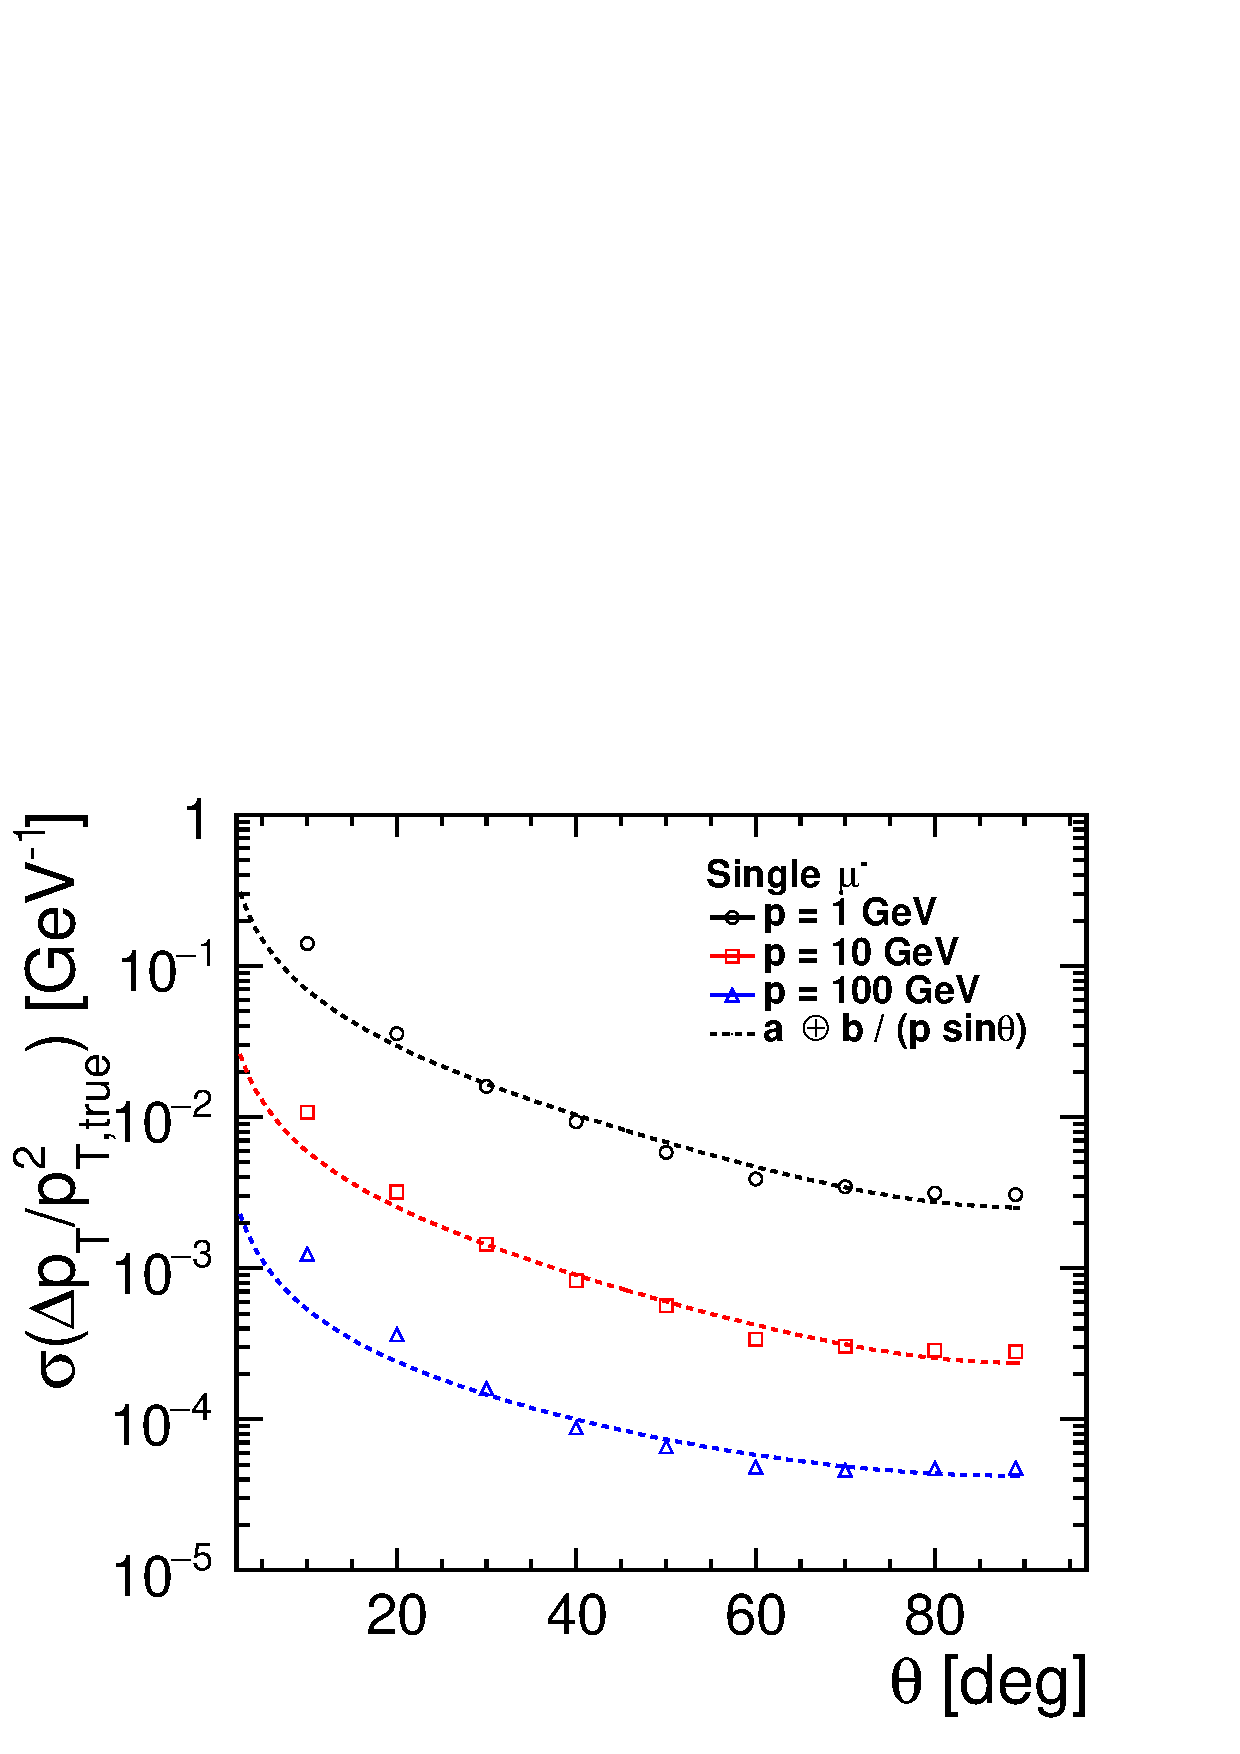
\includegraphics[width=6cm]{fromPreviousTalks/plots_FCCweek_workshop/fromEmilia/MomRes_vs_theta.pdf}};

 \node[inner sep=0pt] (tmp) at (\xRefPosOne-0.2,\yRefPosOne+3.2)
  {\tiny WORK IN PROGRESS};
 \node[inner sep=0pt] (tmp) at (\xRefPosOne+5.99,\yRefPosOne+3.2)
  {\tiny WORK IN PROGRESS};
  
           \node  at (\xRefPosOne-2.9,\yRefPosOne+3.285) (box){%
    \myCenterBox{\small CLICdet}
    };     

       \node  at (\xRefPosOne+3.13,\yRefPosOne+3.285) (box){%
    \myCenterBox{\small CLD }
    };     

  
 \node  at (\xRefPosOne+1,\yRefPosOne+4.3) (box){%
    \begin{minipage}{1.1\textwidth}
      \begin{itemize}
% 		\item Statistics used: 10k single muons at fixed energy and $\theta$ for each datapoint
%         \item Brief look on tracking performance with CLICdet and CLD
        \item Transverse momentum resolution for single muons with CLICdet and CLD detector models as a function of $\theta$ for 1, 10 and 100 GeV energies
      \end{itemize}
    \end{minipage}
  };
  
 \node  at (\xRefPosOne+1,\yRefPosOne-2.5) (box){%
    \begin{minipage}{\textwidth}
      \begin{itemize}
		\item Overall comparable tracking performance of both detectors \\
		\item Achieved momentum resolutions for 100 GeV muons at $\theta =$ 90\degree:
		\begin{itemize}
		 \item 3x10$^{-5}$ GeV$^{-1}$ - CLICdet
		 \item 4x10$^{-5}$ GeV$^{-1}$ - CLD
		\end{itemize}
% 		{\small (CLICdet better at high momentum while CLD better at low momentum tracks)}
      \end{itemize}
    \end{minipage}
  };
 
   
\end{tikzpicture}
\end{frame}
%*****************************************************************************
%*****************************************************************************
% \bgroup
% \setbeamercolor{background canvas}{bg=white}
\begin{frame}{}

    \begin{tikzpicture}[overlay]

    %% HELPER draw advanced helping grid with axises:
%     \draw (0,-5) to[grid with coordinates] (11,3);

    \node[right] (textNode) at (3,0) {
      { \large \bf Particle ID efficiency}
    };
    
    \node[right] (n7) at (4.6,-0.7) {
        \EightStarTaper Single isolated particles
    };
    
    \node[right] (n8) at (4.6,-1.2) {
        \EightStarTaper Leptons in $t\bar{t}$ events
    };

%     \node[right] (n9) at (4.6,-1.7) {
%         \EightStarTaper Efficiency in complex events
%     };
    
    \tikz[overlay]\draw[thick,black,->] ([xshift=-0.6cm]textNode.south) to [out=270, in=180] ([xshift=-0.1pt]n7.west);
    \tikz[overlay]\draw[thick,black,->] ([xshift=-1.1cm]textNode.south) to [out=270, in=180] ([xshift=-0.1pt]n8.west);
%     \tikz[overlay]\draw[thick,black,->] ([xshift=-1.6cm]textNode.south) to [out=270, in=180] ([xshift=-0.1pt]n9.west);    

    \end{tikzpicture}

\end{frame}
% \egroup
%*****************************************************************************

%*****************************************************************************
\begin{frame}{\large \large Single particle identification efficiency}
\renewcommand{\yRefPosOne}{-0.9}
\renewcommand{\xRefPosOne}{4.2}
\renewcommand{\xRefIncrementOne}{7.5}
\begin{tikzpicture}[overlay]

 \node[inner sep=0pt] (tmp) at (\xRefPosOne-1.7,\yRefPosOne-0.6)
%   {\includegraphics[width=6cm]{singleParticleEff/CLD_muon_eff.pdf}};
  {\includegraphics[width=6cm]{may21_muons_eff.pdf}};
  
 \node[inner sep=0pt] (tmp) at (\xRefPosOne+4.5,\yRefPosOne-0.6)
%   {\includegraphics[width=6cm]{singleParticleEff/CLD_pion_eff.pdf}};
  {\includegraphics[width=6cm]{may21_pions_eff.pdf}};


 \node  at (\xRefPosOne+1,\yRefPosOne+3.3) (box){%
    \begin{minipage}{1.1\textwidth}
  \begin{itemize}

   \item Efficiency = fraction of matched reconstructed particles out of the simulated MC particles:
      \begin{itemize}
       \item reconstructed particle of the same type as simulated MC particle
       \item angular matching: $\Delta\theta <$ 1 mrad and $\Delta\phi <$ 2 mrad
       \item energy matching:\\
       - charged particles: $|p_T^{truth} - p_T^{PFO}| < 5\%$ $p_T^{truth} $ \\
       - photons: $\Delta$$E < 5\times\sigma$(ECal) $\approx 0.75\times \sqrt{E}$
      \end{itemize}
    \end{itemize}
    \end{minipage}
  };

  \node [TRTBox]  at (\xRefPosOne+4.8,\yRefPosOne+2.7) (box){%
  \begin{minipage}{0.4\textwidth}
   Sample: single particles with flat cos($\theta$) distribution and fixed energy
  \end{minipage}
  };


  
         \node  at (\xRefPosOne-3.1,\yRefPosOne+1.75) (box){%
    \myCenterBox{\small Muons}
    };     

       \node  at (\xRefPosOne+3,\yRefPosOne+1.75) (box){%
    \myCenterBox{\small Pions}
    };     

 \node[inner sep=0pt] (tmp) at (\xRefPosOne-0.1,\yRefPosOne+1.75)
  {\tiny WORK IN PROGRESS};
 
 \node[inner sep=0pt] (tmp) at (\xRefPosOne+6.1,\yRefPosOne+1.75)
  {\tiny WORK IN PROGRESS};
    
 \node  at (\xRefPosOne+1,\yRefPosOne-3.5) (box){%
    \begin{minipage}{\textwidth}
      \begin{itemize}
        \item $>$99$\%$ muon efficiency and 93-96$\%$ pion efficiency for E$>$10 GeV
        \item Inefficiency at high energies with CLD is caused by a larger rate of pions being mis-reconstructed as muons 
%         $\to$ optimization of muon requirements are needed
      \end{itemize}
    \end{minipage}
  };
 
 \end{tikzpicture}
\end{frame}
%*****************************************************************************
%*****************************************************************************
\begin{frame}{\large \large Single particle identification efficiency}
\renewcommand{\yRefPosOne}{-0.5}
\renewcommand{\xRefPosOne}{4.2}
\renewcommand{\xRefIncrementOne}{7.5}
\begin{tikzpicture}[overlay]

 \node[inner sep=0pt] (tmp) at (\xRefPosOne-1.7,\yRefPosOne-0.6)
  {\includegraphics[width=6cm]{may21_photon_eff.pdf}}; 
  
 \node[inner sep=0pt] (tmp) at (\xRefPosOne+4.5,\yRefPosOne-0.6)
  {\includegraphics[width=6cm]{may21_electron_eff.pdf}};


 \node  at (\xRefPosOne+1,\yRefPosOne+2.9) (box){%
    \begin{minipage}{1.15\textwidth}
  \begin{itemize}

   \item Photon merging procedure is used to recover inefficiency due to photon conversion and electron Bremsstrahlung
   \item Pandora electron ID parameters were retuned in order to recover  hard electron Bremsstrahlung \\ {\small (loosen maximum track-cluster distance requirement to recover events when a track is not associated to either of EM clusters)}
    \end{itemize}
    \end{minipage}
  };


 \node  at (\xRefPosOne+1,\yRefPosOne-3.7) (box){%
    \begin{minipage}{\textwidth}
      \begin{itemize}
        \item $>95\%$ efficiency for $>$10 GeV photons and $>$20 GeV electrons  
        \item Further optimization of electron Bremsstrahlung recovery procedure may improve electron efficiency (e.g. at lower energies)
%         {\tiny [TODO electron plot has to be updated]}
      \end{itemize}
    \end{minipage}
  };
   
       \node  at (\xRefPosOne-3,\yRefPosOne+1.75) (box){%
    \myCenterBox{\small Photons}
    };     

       \node  at (\xRefPosOne+3.25,\yRefPosOne+1.75) (box){%
    \myCenterBox{\small Electrons}
    };     

 \node[inner sep=0pt] (tmp) at (\xRefPosOne-0.1,\yRefPosOne+1.75)
  {\tiny WORK IN PROGRESS};
 
 \node[inner sep=0pt] (tmp) at (\xRefPosOne+6.1,\yRefPosOne+1.75)
  {\tiny WORK IN PROGRESS};
    
 \end{tikzpicture}
\end{frame}
%*****************************************************************************
%*****************************************************************************
\begin{frame}{\large \large Lepton identification efficienty in $t\bar{t}$ events at CLIC}
\renewcommand{\yRefPosOne}{0}
\renewcommand{\xRefPosOne}{4.2}
\renewcommand{\xRefIncrementOne}{7.5}
\begin{tikzpicture}[overlay]

 \node[inner sep=0pt] (tmp) at (\xRefPosOne-1.7,\yRefPosOne-0.6)
  {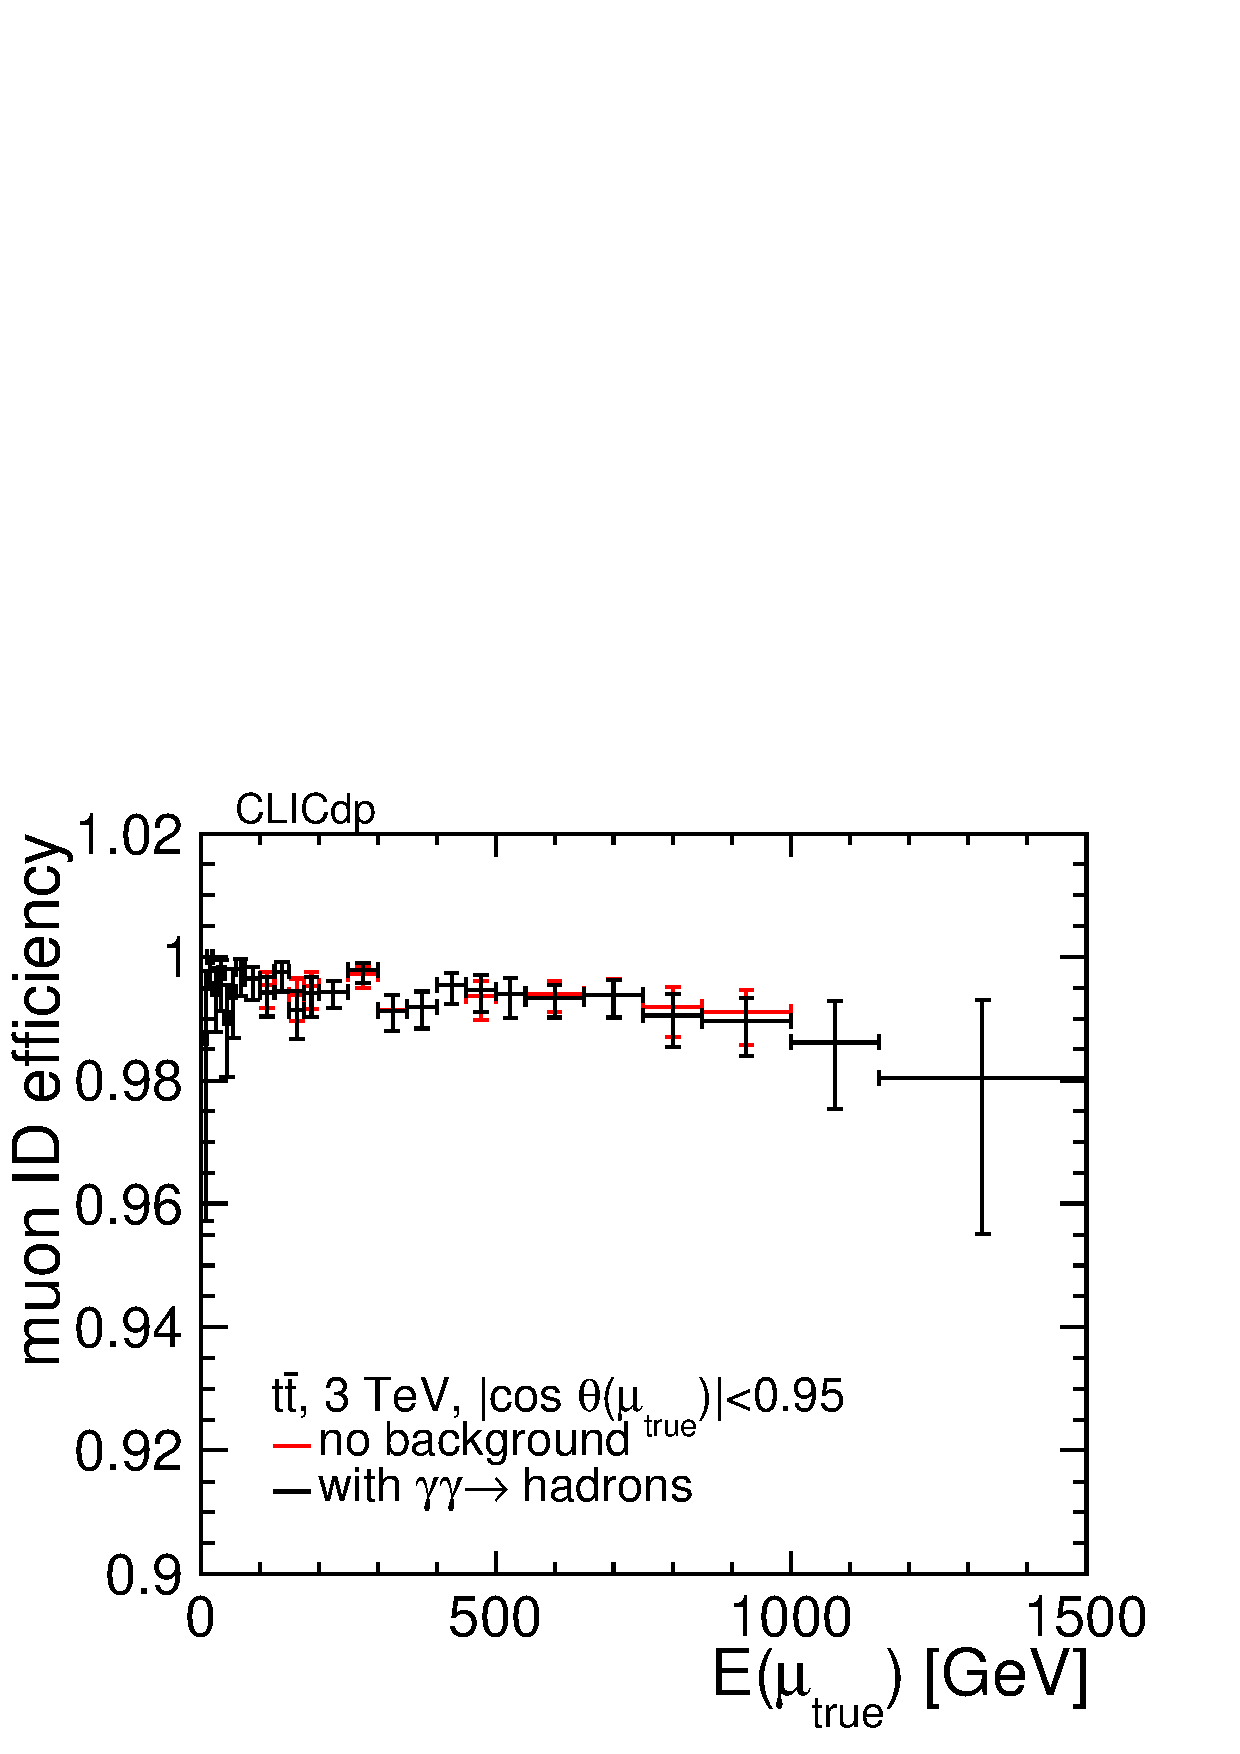
\includegraphics[width=6cm]{MuEff_vs_trueMu_E_ttbar_3TeV_cos_0_95.pdf}}; 
  
 \node[inner sep=0pt] (tmp) at (\xRefPosOne+4.5,\yRefPosOne-0.6)
  {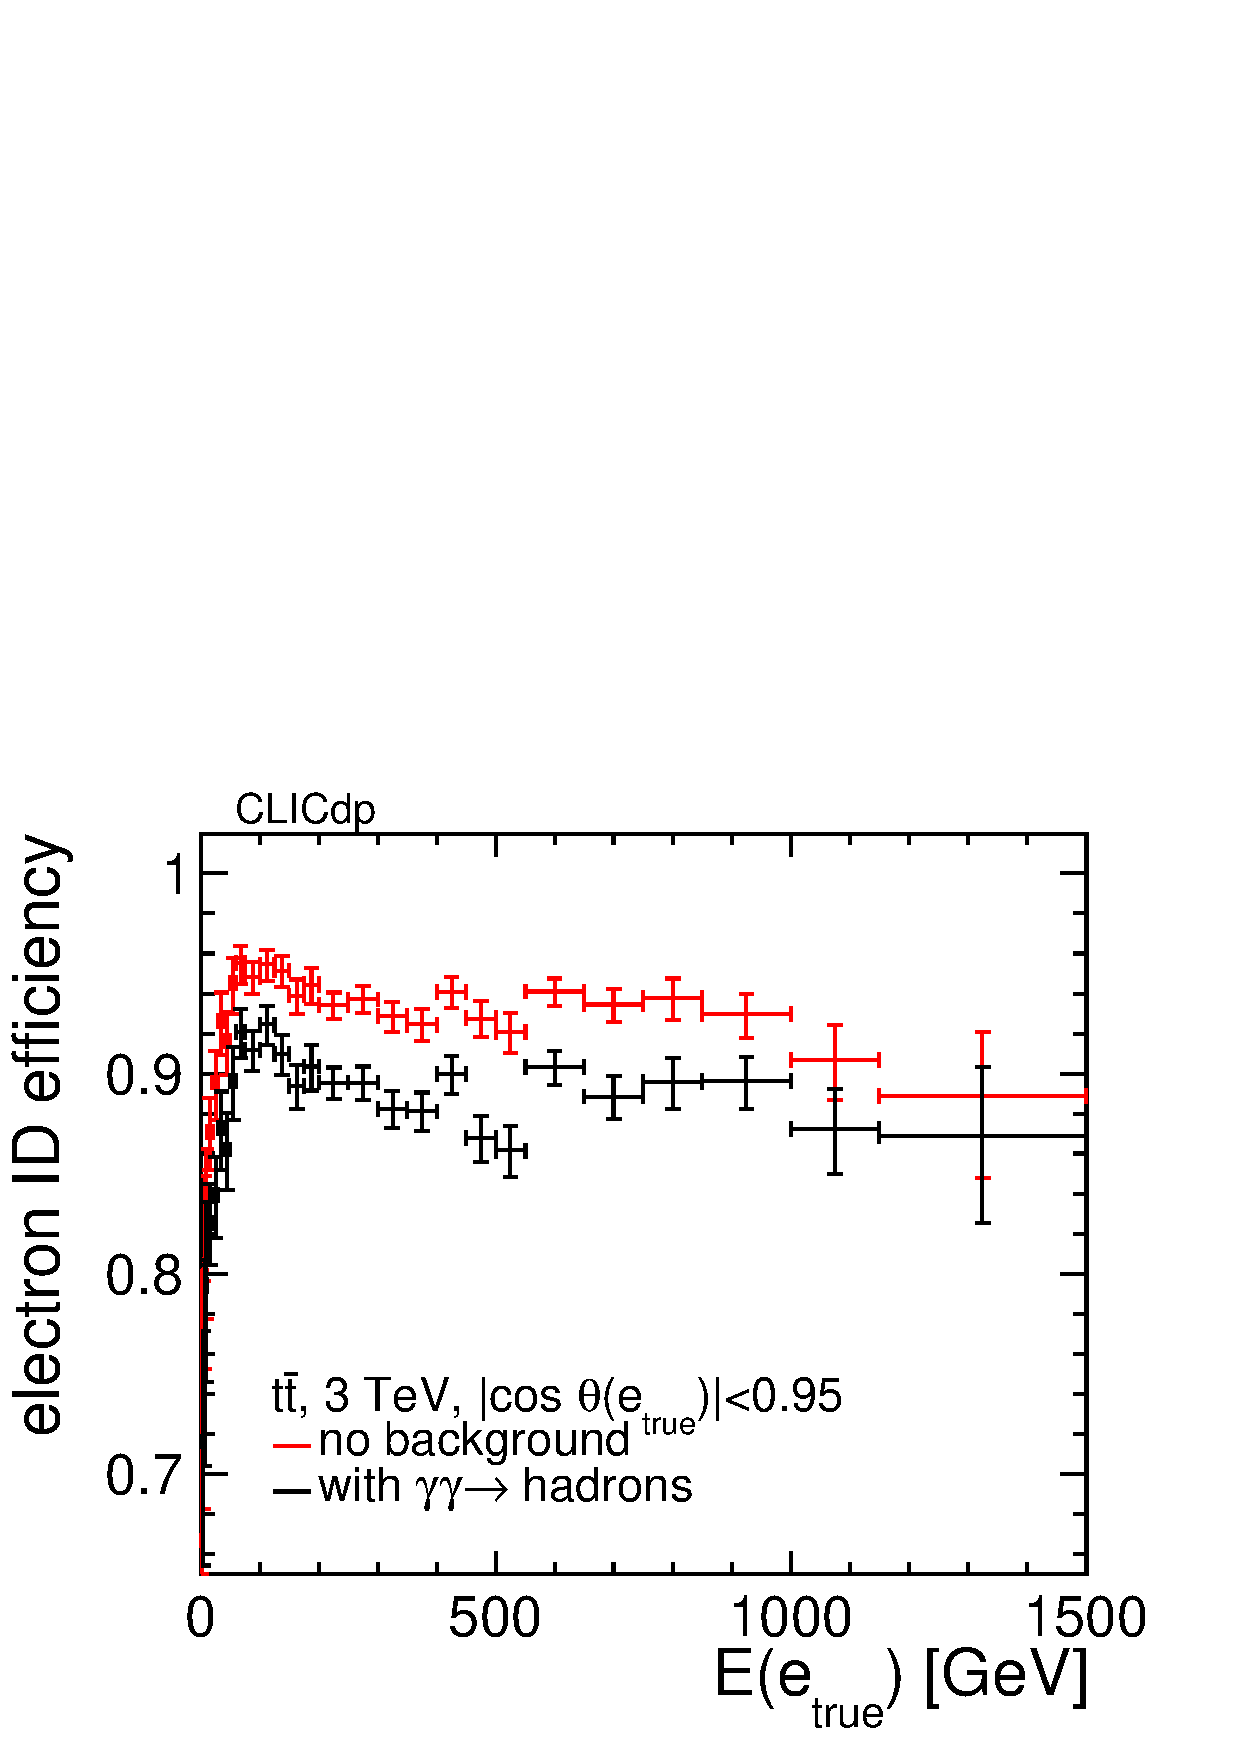
\includegraphics[width=6cm]{ElEff_vs_trueEl_E_ttbar_3TeV_cos_0_95.pdf}};


 \node  at (\xRefPosOne+1,\yRefPosOne+2.8) (box){%
    \begin{minipage}{1.1\textwidth}
  \begin{itemize}

   \item Lepton ID efficiency in $t\bar{t}$ events at 3 TeV at CLIC
   \item Only direct leptons from W decays are considered
   \item Requirement of angular matching within 1\degree is imposed.
    \end{itemize}
    \end{minipage}
  };


 \node  at (\xRefPosOne+1,\yRefPosOne-4) (box){%
    \begin{minipage}{\textwidth}
      \begin{itemize}
        \item Muons are identified with more than 98$\%$ efficiency for all energies
        \item Electrons are identified with 90-95$\%$ efficiency at energies of 20 GeV and higher
        \item Presence of beam background doesn't affect muon ID while electron ID decreases by about 5$\%$
%         {\tiny [TODO electron plot has to be updated]}
      \end{itemize}
    \end{minipage}
  };
   
       \node  at (\xRefPosOne-3.1,\yRefPosOne+1.75) (box){%
    \myCenterBox{\small Muons}
    };     

       \node  at (\xRefPosOne+3.25,\yRefPosOne+1.75) (box){%
    \myCenterBox{\small Electrons}
    };     

 \node[inner sep=0pt] (tmp) at (\xRefPosOne-0.1,\yRefPosOne+1.75)
  {\tiny WORK IN PROGRESS};
 
 \node[inner sep=0pt] (tmp) at (\xRefPosOne+6.1,\yRefPosOne+1.75)
  {\tiny WORK IN PROGRESS};
    
 \end{tikzpicture}
\end{frame}
%*****************************************************************************
%*****************************************************************************
% \bgroup
% \setbeamercolor{background canvas}{bg=white}
\begin{frame}{}

    \begin{tikzpicture}[overlay]

    %% HELPER draw advanced helping grid with axises:
%     \draw (0,-5) to[grid with coordinates] (11,3);

    \node[right] (textNode) at (3,0) {
      { \large \bf Jet performance}
    };
    
    \node[right] (n7) at (4.6,-0.7) {
        \EightStarTaper Software compensation
    };
    
    \node[right] (n8) at (4.6,-1.2) {
        \EightStarTaper Jet Energy Resolution 
    };

%     \node[right] (n9) at (4.6,-1.7) {
%         \EightStarTaper Efficiency in complex events
%     };
    
    \tikz[overlay]\draw[thick,black,->] ([xshift=-0.6cm]textNode.south) to [out=270, in=180] ([xshift=-0.1pt]n7.west);
    \tikz[overlay]\draw[thick,black,->] ([xshift=-1.1cm]textNode.south) to [out=270, in=180] ([xshift=-0.1pt]n8.west);
%     \tikz[overlay]\draw[thick,black,->] ([xshift=-1.6cm]textNode.south) to [out=270, in=180] ([xshift=-0.1pt]n9.west);    

    \end{tikzpicture}

\end{frame}
% \egroup
%*****************************************************************************
%*****************************************************************************
\begin{frame}{\large \large Software Compensation}
\renewcommand{\yRefPosOne}{0}
\renewcommand{\xRefPosOne}{5.3}
\renewcommand{\xRefIncrementOne}{5.5}

 \begin{tikzpicture}[overlay]
 
%   \node[inner sep=0pt] (tmp) at (\xRefPosOne,\yRefPosOne+0.5)
%     {\includegraphics[width=8cm]{Matthias/ClosurePlotOfHighEnergyRangeNeutrons.pdf}};

 \node[inner sep=0pt] (tmp) at (\xRefPosOne+3.5,\yRefPosOne-2.0)
    {\includegraphics[width=5cm]{fromPreviousTalks/swComp_weights_example.png}};
 
 
 
 \node  at (\xRefPosOne-2.7,\yRefPosOne-1.8) (box){%
    \begin{minipage}{0.6\textwidth}
    Software compensation:
  \begin{itemize}
   \item Electromagnetic component of shower typically denser
   \item Software compensation reweights hits in HCAL depending on the hit energy
density
    \item Weights are calculated by formula: $\omega(\rho) = $p$_1 $exp$($p$_2 \rho) + $p$_3$ \\[0.1cm]
    where each parameter is an energy dependent\\ $\to$
    9 different parameters are used in total
    
%    \item In total 9 different parameters are used
%    \item Weight includes an energy dependence
   
  \end{itemize}
    \end{minipage}
};

\node  at (\xRefPosOne-0.6,\yRefPosOne+1.8) (box){%
    \begin{minipage}{1.05\textwidth}
%     Nonlinear non compensating natures of hadron calorimeters:
  \begin{itemize}
    \item Software compensation is an energy ``regularisation'' techniques ({\small  \href{http://iopscience.iop.org/1748-0221/7/09/P09017}{\color{blue}JINST 7 (2012) P09017}})
   \item Idea is to correct with software for (on average) larger response of hadron
showers with large electromagnetic component $\to$ improves energy
measurement of cluster energies
   \item Software compensation technique (developed by CALICE) is implemented in
PandoraPFA now
  \end{itemize}
    \end{minipage}
};

\node [PixelBox] at (\xRefPosOne-2.3,\yRefPosOne-4.2) (box){%
  \begin{minipage}{0.55\textwidth}
  Detector specific software compensation weights were obtained for CLICdet and CLD 
  \end{minipage}
};

% \node [PixelBox] at (\xRefPosOne,\yRefPosOne-4) (box){%
%   \begin{minipage}{\textwidth}
%   Default weight tuned for ILD experiment at ILC up to 100 GeV, at CLIC expect to
% reach higher hadron energies, at 3 TeV sometimes beyond 500 GeV
% $\to$ retune parameters for CLIC ({\small Follow description of paper EPJC 77 (2017) 698})
%   \end{minipage}
% };

\node  at (\xRefPosOne+4.95,\yRefPosOne+0.63) (box){%
\myVerySmallCenterBox[TRTColor]{EPJC 77 (2017) 698}
}; 





\end{tikzpicture}
 
\end{frame}
%*****************************************************************************
%*****************************************************************************
\begin{frame}{\large \large Hadron response with Software Compensation}
\renewcommand{\yRefPosOne}{0}
\renewcommand{\xRefPosOne}{5.3}
\renewcommand{\xRefIncrementOne}{5.5}

 \begin{tikzpicture}[overlay]
 
  \node[inner sep=0pt] (tmp) at (\xRefPosOne,\yRefPosOne+0.5)
    {\includegraphics[width=8cm]{fromPreviousTalks/ClosurePlotOfHighEnergyRangeNeutrons.pdf}};

 
 \node  at (\xRefPosOne,\yRefPosOne-3.5) (box){%
    \begin{minipage}{\textwidth}

  \begin{itemize}
%    \item Software compensation weights derived from MC using neutron and $K_L^0$ events
  \item Software compensation weights derived using several fully simulated neutron and K0L single particle datasets
   \item Mean and resolution after software compensation largely improved
   \item Software compensation corrects for nonlinear response of hadrons on the fly
  \end{itemize}

    \end{minipage}
};

\end{tikzpicture}
 
\end{frame}
%*****************************************************************************

%*****************************************************************************
\begin{frame}{\large \large Total reconstructed energy in dijet events with Software Compensation}
\renewcommand{\yRefPosOne}{0}
\renewcommand{\xRefPosOne}{5.3}
\renewcommand{\xRefIncrementOne}{5.5}

 \begin{tikzpicture}[overlay]
 
 
  \node  at (\xRefPosOne+0.4,\yRefPosOne+2.85) (box){%
    \begin{minipage}{1.1\textwidth}
  \begin{itemize}
  \item Dijet events of a Z-like particle decaying into pair of light quarks (u, d, s) at several centre-of-mass energies
    \end{itemize}
    \end{minipage}
  };
 
  \node[inner sep=0pt] (tmp) at (\xRefPosOne,\yRefPosOne-0.4)
    {\includegraphics[width=7cm]{matthias_SWC_linearity.pdf}};
 
         \node[inner sep=0pt] (tmp) at (\xRefPosOne-1.0,\yRefPosOne+2.25)
  {\tiny  \textbf{CLICdp WORK IN PROGRESS}};
 
 \node  at (\xRefPosOne,\yRefPosOne-3.8) (box){%
    \begin{minipage}{\textwidth}
  \begin{itemize}
  \item Ratio of total reconstructed energy to total simulated energy (excluding neutrinos)
  \item Software compensation provides reconstruction of total energy within 0.5$\%$ accuracy in light-quark dijet sample.
  \end{itemize}

    \end{minipage}
};

\end{tikzpicture}
 
\end{frame}
%*****************************************************************************
%*****************************************************************************
\begin{frame}{\large \large Jet energy resolution with dijet events}

\renewcommand{\yRefPosOne}{-1.5}
\renewcommand{\xRefPosOne}{5.3}
\renewcommand{\xRefIncrementOne}{5.5}
\begin{tikzpicture}[overlay]

  \node  at (\xRefPosOne+0.4,\yRefPosOne+4.5) (box){%
    \begin{minipage}{1.1\textwidth}
  \begin{itemize}
  \item Dijet events of a Z-like particle decaying into pair of light quarks (u, d, s) at several centre-of-mass energies
    \end{itemize}
    \end{minipage}
  };

 \node[inner sep=0pt] (tmp) at (\xRefPosOne-2.7,\yRefPosOne+1.2)
    {\includegraphics[width=6cm]{JER_FCCee_vs_CLIC_conformal_Zuds91_matthiasCLIC.pdf}};
    
 \node[inner sep=0pt] (tmp) at (\xRefPosOne+3.3,\yRefPosOne+1.2)
    {\includegraphics[width=6cm]{JER_FCCee_vs_CLIC_conformal_Zuds380_matthiasCLIC.pdf}};
    
 \node[inner sep=0pt] (tmp) at (\xRefPosOne-3.6,\yRefPosOne+3.5)
    {\tiny WORK IN PROGRESS};
 \node[inner sep=0pt] (tmp) at (\xRefPosOne+2.4,\yRefPosOne+3.5)
    {\tiny WORK IN PROGRESS};
    
\node  at (\xRefPosOne-1.13,\yRefPosOne+3.55) (box){%
\myCenterBox{\small 45.5 GeV jets}
}; 

\node  at (\xRefPosOne+4.9,\yRefPosOne+3.55) (box){%
\myCenterBox{\small 190 GeV jets}
}; 



\node  at (\xRefPosOne,\yRefPosOne-2.3) (box){%
\begin{minipage}{\textwidth}
  \begin{itemize}
   \item Comparable resolution for both detectors
    \item Jet energy resolution in barrel region:
    \begin{itemize}
        \item 45.5 GeV jets: 4-5 $\%$
        \item 190 GeV jets: 3-4 $\%$ \\ [0.2cm]
    \end{itemize}
  \end{itemize}
\end{minipage}
};

  \node [PixelBox, inner sep=4pt]  at (\xRefPosOne+3.55,\yRefPosOne-2.4) (box){%
    \begin{minipage}{0.45\textwidth}
    \small
		Jet energy (E$_j$) is measured as a half of total energy (E$_{jj}$) of Z$\to q\bar{q}$ (q=u,d,s) di-jet event\\
		
		\hspace{0.4cm}
		  {\includegraphics[width=4cm]{../plots_FCCweek_workshop/other/jetRes_formula.png}}
		
    \end{minipage}
  };

% % HELPER draw advanced helping grid with axises:
% \draw(-0.5,-4) to[grid with coordinates] (11.5,4);
\end{tikzpicture}
 
\end{frame}
%*****************************************************************************
%*****************************************************************************
\begin{frame}{\large \large Jet energy resolution at CLIC at high energies}

\renewcommand{\yRefPosOne}{-0.5}
\renewcommand{\xRefPosOne}{5.3}
\renewcommand{\xRefIncrementOne}{5.5}
\begin{tikzpicture}[overlay]

 \node[inner sep=0pt] (tmp) at (\xRefPosOne,\yRefPosOne+1.15)
    {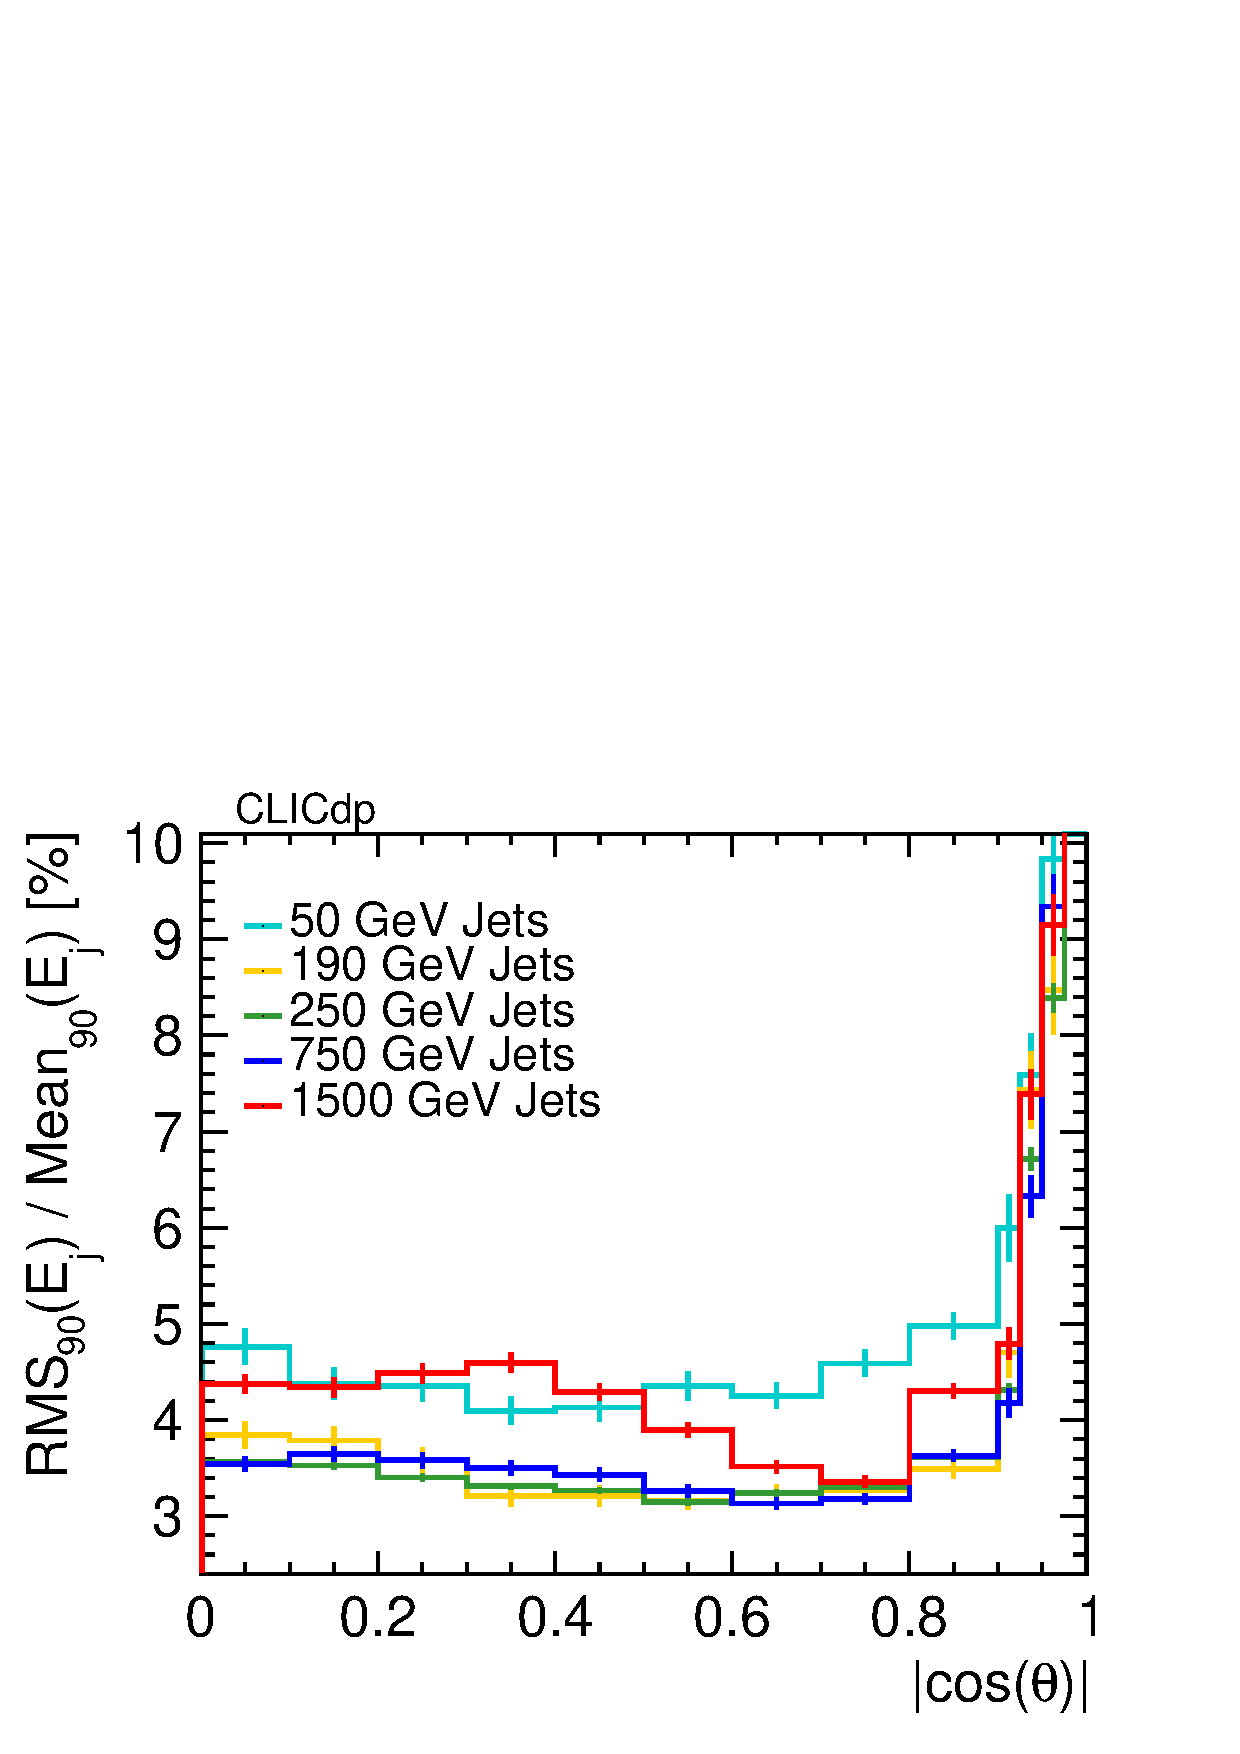
\includegraphics[width=7cm]{JER_RMS90_vs_CosTheta_ILC171221_CT_100_3000.pdf}};
    
%  \node[inner sep=0pt] (tmp) at (\xRefPosOne+3.3,\yRefPosOne+1.2)
%     {\includegraphics[width=6cm]{JER_FCCee_vs_CLIC_conformal_Zuds380_matthiasCLIC.pdf}};
%     
 \node[inner sep=0pt] (tmp) at (\xRefPosOne+2,\yRefPosOne+3.75)
    {\tiny WORK IN PROGRESS};
%  \node[inner sep=0pt] (tmp) at (\xRefPosOne+2.4,\yRefPosOne+3.5)
%     {\tiny WORK IN PROGRESS};
    
% \node  at (\xRefPosOne-1.13,\yRefPosOne+3.55) (box){%
% \myCenterBox{\small 45.5 GeV jets}
% }; 
% 
% \node  at (\xRefPosOne+4.9,\yRefPosOne+3.55) (box){%
% \myCenterBox{\small 190 GeV jets}
% }; 



\node  at (\xRefPosOne,\yRefPosOne-2.8) (box){%
\begin{minipage}{\textwidth}
  \begin{itemize}
   \item Default Software compensation are tuned for hadrons up to 100 GeV ({\small optimized for ILD detector at ILC}), at CLIC expect to reach higher hadron energies, at 3 TeV sometimes beyond 500 GeV $\to$ extend applicability range and retune for CLIC
   \item Excellent jet energy resolution (3.5-4.5 $\%$) for most jet energies up to the endcaps ($|$cos($\theta$)$| >$ 0.925)
   \item Conformal tracking is not yet fully efficient at 1500 GeV and  work is ongoing $\to$ jet energy resolution is expected to become better 

  \end{itemize}
\end{minipage}
};


% % HELPER draw advanced helping grid with axises:
% \draw(-0.5,-4) to[grid with coordinates] (11.5,4);
\end{tikzpicture}
 
\end{frame}
%*****************************************************************************
%*****************************************************************************
\begin{frame}{\large \large Jet energy resolution with and w/o Software compensation}

\renewcommand{\yRefPosOne}{-0.5}
\renewcommand{\xRefPosOne}{5.3}
\renewcommand{\xRefIncrementOne}{5.5}
\begin{tikzpicture}[overlay]

 \node[inner sep=0pt] (tmp) at (\xRefPosOne-2.7,\yRefPosOne+1.2)
    {\includegraphics[width=6cm]{JER_SWC_ON_and_OFF_conformal_Zuds1000_matthiasCLIC.pdf}};
    
 \node[inner sep=0pt] (tmp) at (\xRefPosOne+3.3,\yRefPosOne+1.2)
    {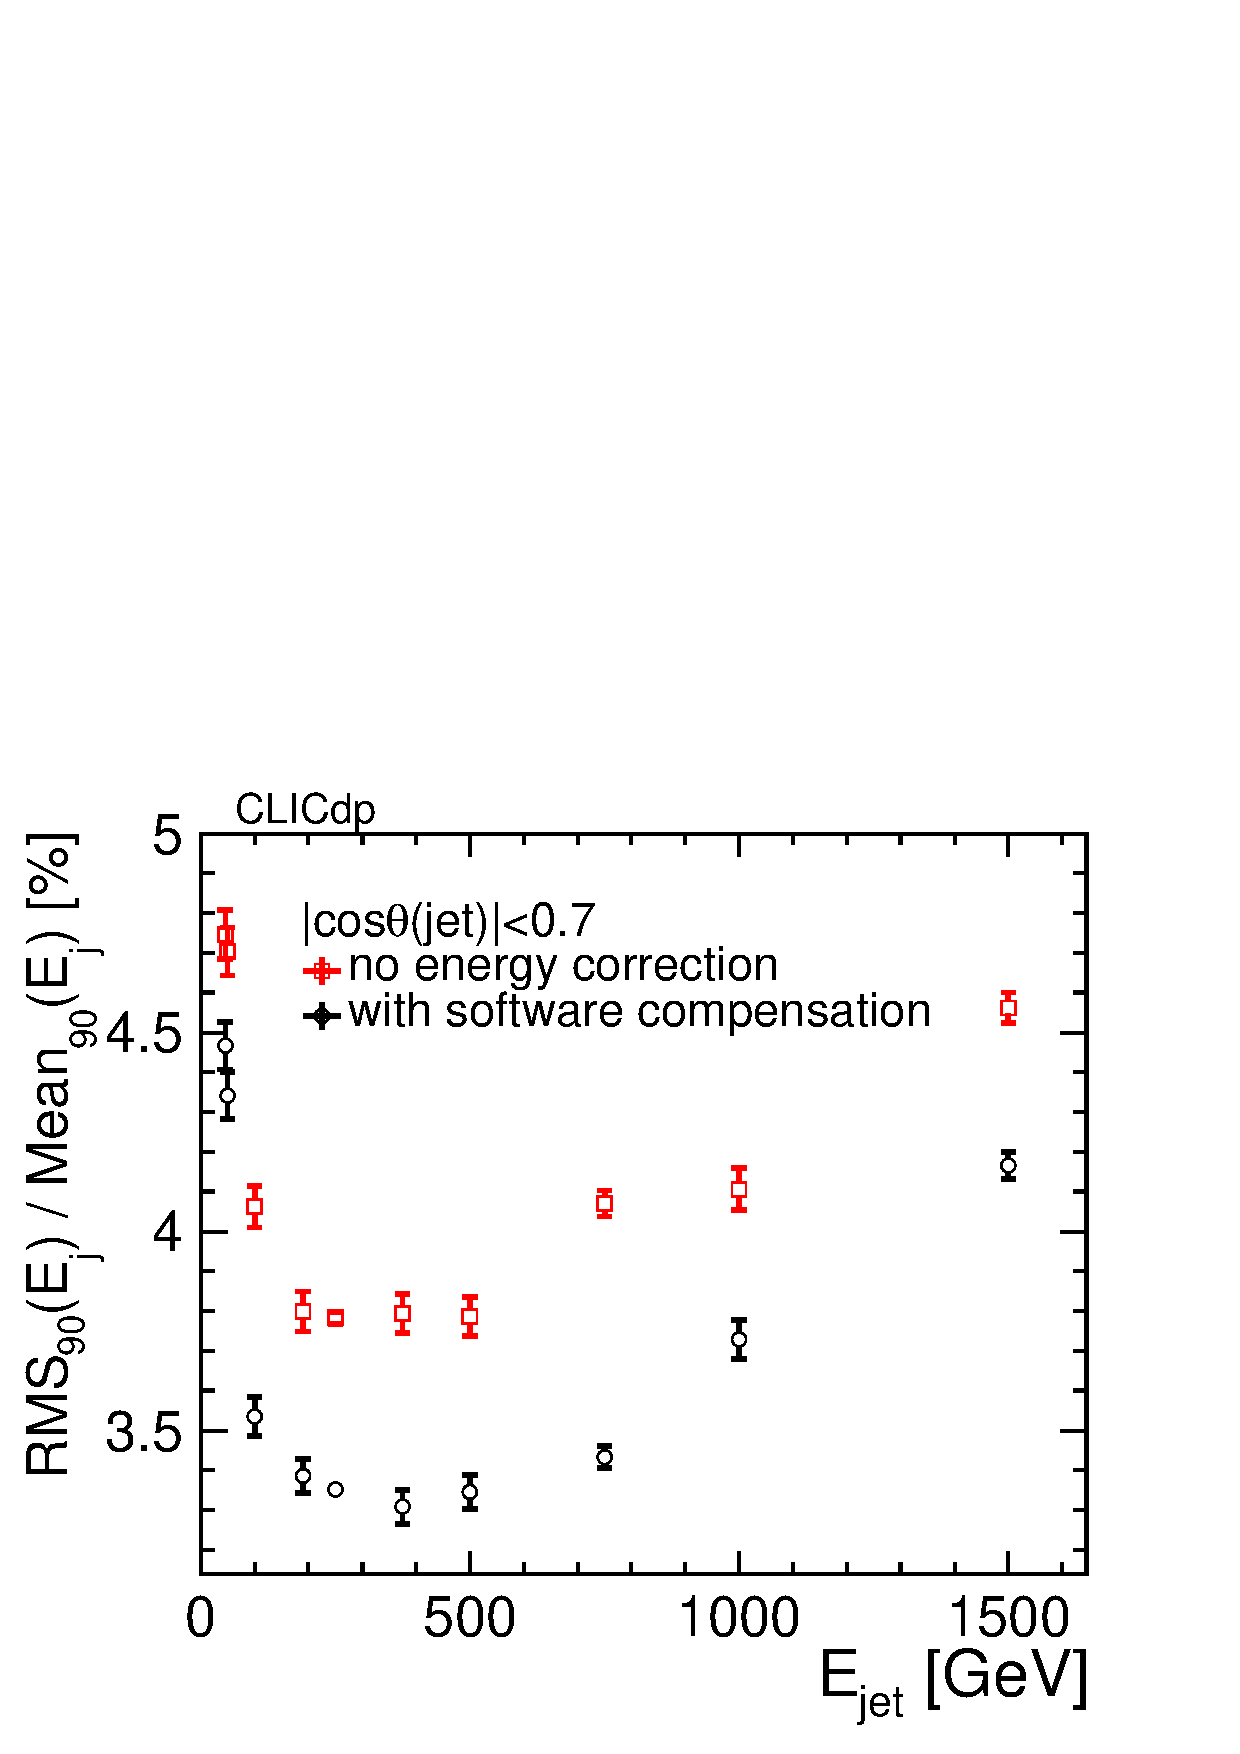
\includegraphics[width=6cm]{JER_RMS90_vs_E_ILC171221_SC_vs_noSC_90_3000.pdf}};
    
 \node[inner sep=0pt] (tmp) at (\xRefPosOne-3.9,\yRefPosOne+3.5)
    {\tiny WORK IN PROGRESS};
 \node[inner sep=0pt] (tmp) at (\xRefPosOne+4.9,\yRefPosOne+3.5)
    {\tiny WORK IN PROGRESS};
    
% \node  at (\xRefPosOne-1.13,\yRefPosOne+3.55) (box){%
% \myCenterBox{\small 190 GeV jets}
% }; 
 
\node  at (\xRefPosOne-1.22,\yRefPosOne+3.53) (box){%
\myCenterBox{\tiny CLICdet, 1.0 TeV jets} 
}; 



\node  at (\xRefPosOne,\yRefPosOne-2.8) (box){%
\begin{minipage}{\textwidth}
  \begin{itemize}
   \item Software compensation improves jet energy resolution within the whole $\theta$ range in all energies
   \item Improvement reaches 10-25 $\%$ in barrel region 
    \item Software compensation performs well even with high jet energies 
  \end{itemize}
\end{minipage}
};


% % HELPER draw advanced helping grid with axises:
% \draw(-0.5,-4) to[grid with coordinates] (11.5,4);
\end{tikzpicture}
 
\end{frame}
%*****************************************************************************
%*****************************************************************************
\begin{frame}{\large \large Summary}
 
 \renewcommand{\yRefPosOne}{0}
\renewcommand{\xRefPosOne}{5.3}
\renewcommand{\xRefIncrementOne}{5.5}
\begin{tikzpicture}[overlay]

       
\node  at (\xRefPosOne,\yRefPosOne+2) (box){%
  \begin{minipage}{0.99\textwidth}
  Performance of CLICdet and CLD detectors have been studied with PandoraPFA with isolated single particles and dijet events:  
 \begin{itemize}
  
  \item Good single particle ID efficiency for both detectors \\ ($>$95$\%$ from 20 GeV for charged particles)
  \item Excellent jet energy resolution (3.5-4.5 $\%$) for most jet energies up to the endcaps 
    \end{itemize}
  \end{minipage}
};

\node at (\xRefPosOne,\yRefPosOne) (box){%
  \begin{minipage}{0.99\textwidth}
Overall calorimetry performance of CLD detector (FCCee) is similar to CLICdet
  \end{minipage}
};

\node at (\xRefPosOne,\yRefPosOne-2) (box){%
  \begin{minipage}{0.99\textwidth}
Software compensation:
 \begin{itemize}
  \item improves jet energy resolution by 10-25$\%$
  \item provides reconstruction of total energy in dijet events with accuracy of 0.5$\%$
  \item performs well even at high jet energies (tested up to 3 TeV centre-of-mass-energy)
    \end{itemize}
  \end{minipage}
};

\node[right] (textNode) at (3,-4) {
      { \large \bf Thank you for your attention! }
    };

\end{tikzpicture}
  
\end{frame}
%*****************************************************************************
\backupbegin
%*****************************************************************************
\begin{frame}
\frametitle{BACKUP} 
 
\end{frame}
%*****************************************************************************
%*****************************************************************************
\begin{frame}{\large \large CLD vs CLICdet dimensions}
 
\renewcommand{\yRefPosOne}{0}
\renewcommand{\xRefPosOne}{5.3}
\renewcommand{\xRefIncrementOne}{5.5}
\begin{tikzpicture}[overlay]


 \node[TRTBox] (tmp) at (\xRefPosOne,\yRefPosOne-0.5)
  { 
    \begin{minipage}{0.8\textwidth}

    \resizebox{\columnwidth}{!}{%
      \begin{tabular}{lccc}
	 & CLICdet & & CLD \\[0.18cm]
	VTX Barrel & 31-60 mm & $\Longrightarrow$ & 17-59 mm \\[0.18cm]
	VTX Endcap & Spirals & $\Longrightarrow$ & Disks \\[0.18cm]
	Tracker radius & 1486 mm & $\Longrightarrow$ & 2100 mm \\[0.18cm]
% 	ECAL thickness & 202 mm & $\Longrightarrow$ & 202 mm \\[0.18cm]
% 	HCAL thickness & 44 $\times$ 7.5 $\lambda_0$ & $\Longrightarrow$ & 44 $\times$ 5.5 $\lambda_0$ \\[0.18cm]
	ECAL thickness & 40 layers, 22 X$_0$ & $\Longrightarrow$ & 40 layers, 22 X$_0$ \\[0.18cm]
	HCAL thickness & 60 layers, 7.5 $\lambda_I$ & $\Longrightarrow$ & 44 layers, 5.5 $\lambda_I$ \\[0.18cm]
	Yoke thickness & 1989 mm & $\Longrightarrow$ & 1521 mm \\[0.18cm]
	MDI (forward region) &  & $\Longrightarrow$ & $<$ 150 mrad \\[0.4cm]
	Solenoid field & 4 Tesla & $\Longrightarrow$ & 2 Tesla \\
	
      \end{tabular}%
    }
    \end{minipage}
  };
  


\node at (\xRefPosOne,\yRefPosOne+2.6) (box){%
\myCenterBox[TRTColor]{Overall dimensions of CLIC and FCC-ee detectors}
};
  
\end{tikzpicture}
\end{frame}
%*****************************************************************************
%*****************************************************************************
\begin{frame}{\large \large Pion identification efficiency}
\renewcommand{\yRefPosOne}{-0.5}
\renewcommand{\xRefPosOne}{4.2}
\renewcommand{\xRefIncrementOne}{7.5}
\begin{tikzpicture}[overlay]

 \node[inner sep=0pt] (tmp) at (\xRefPosOne-1.7,\yRefPosOne-0.6)
  {\includegraphics[width=6cm]{../plots_FCCweek_workshop/singleParticleEff/pion_eff_vs_theta_E20.pdf}}; 
  
 \node[inner sep=0pt] (tmp) at (\xRefPosOne+4.5,\yRefPosOne-0.6)
  {\includegraphics[width=6cm]{../plots_FCCweek_workshop/singleParticleEff/pion_eff_vs_theta_E100.pdf}};


 \node  at (\xRefPosOne+1,\yRefPosOne+2.9) (box){%
    \begin{minipage}{1.1\textwidth}
  \begin{itemize}

   \item Pion ID efficiency and inefficiency as function of cos($\theta$)
    \end{itemize}
    \end{minipage}
  };


 \node  at (\xRefPosOne+1,\yRefPosOne-3.5) (box){%
    \begin{minipage}{\textwidth}
      \begin{itemize}
        \item High momentum pions more often are misreconstructed as muons in barrel
      \end{itemize}
    \end{minipage}
  };
   
       \node  at (\xRefPosOne-2.65,\yRefPosOne+1.75) (box){%
    \myCenterBox{\small 20 GeV pions}
    };     

       \node  at (\xRefPosOne+3.6,\yRefPosOne+1.75) (box){%
    \myCenterBox{\small 100 GeV pions}
    };     

 \node[inner sep=0pt] (tmp) at (\xRefPosOne-0.1,\yRefPosOne+1.75)
  {\tiny WORK IN PROGRESS};
 
 \node[inner sep=0pt] (tmp) at (\xRefPosOne+6.1,\yRefPosOne+1.75)
  {\tiny WORK IN PROGRESS};
    
 \end{tikzpicture}
\end{frame}
%*****************************************************************************
%*****************************************************************************
\begin{frame}{\large \large Electron identification efficiency}
\renewcommand{\yRefPosOne}{-0.5}
\renewcommand{\xRefPosOne}{4.2}
\renewcommand{\xRefIncrementOne}{7.5}
\begin{tikzpicture}[overlay]

 \node[inner sep=0pt] (tmp) at (\xRefPosOne-1.7,\yRefPosOne-0.6)
  {\includegraphics[width=6cm]{../plots_FCCweek_workshop/singleParticleEff/electron_eff_vs_theta_E20.pdf}}; 
  
 \node[inner sep=0pt] (tmp) at (\xRefPosOne+4.5,\yRefPosOne-0.6)
  {\includegraphics[width=6cm]{../plots_FCCweek_workshop/singleParticleEff/electron_eff_vs_theta_E100.pdf}};


 \node  at (\xRefPosOne+1,\yRefPosOne+2.9) (box){%
    \begin{minipage}{1.1\textwidth}
  \begin{itemize}

   \item Electron ID efficiency and inefficiency as function of cos($\theta$)
    \end{itemize}
    \end{minipage}
  };


 \node  at (\xRefPosOne+1,\yRefPosOne-3.5) (box){%
    \begin{minipage}{\textwidth}
      \begin{itemize}
        \item Inefficiency for high-momentum electrons can be recovered by better Bremsstrahlung recovery algorithm
      \end{itemize}
    \end{minipage}
  };
   
       \node  at (\xRefPosOne-2.5,\yRefPosOne+1.75) (box){%
    \myCenterBox{\small 20 GeV electrons}
    };     

       \node  at (\xRefPosOne+3.75,\yRefPosOne+1.75) (box){%
    \myCenterBox{\small 100 GeV electrons}
    };     

 \node[inner sep=0pt] (tmp) at (\xRefPosOne-0.1,\yRefPosOne+1.75)
  {\tiny WORK IN PROGRESS};
 
 \node[inner sep=0pt] (tmp) at (\xRefPosOne+6.1,\yRefPosOne+1.75)
  {\tiny WORK IN PROGRESS};
    
 \end{tikzpicture}
\end{frame}
%*****************************************************************************
%*****************************************************************************
\begin{frame}{\large \large Electron identification efficiency (Pandora track-cluster association algorithm)}

\renewcommand{\yRefPosOne}{-0.5}
\renewcommand{\xRefPosOne}{5.5}
\renewcommand{\xRefIncrementOne}{5.5}
\begin{tikzpicture}[overlay]

 \node[inner sep=0pt] (tmp) at (\xRefPosOne-3,\yRefPosOne+1.2)
    {\includegraphics[width=6.2cm]{../plots_FCCweek_workshop/other/calice_CLIC_vs_FCCee_effVsTheta_fakes_electrons_E10.pdf}};
    
 \node[inner sep=0pt] (tmp) at (\xRefPosOne+3,\yRefPosOne-0.1)
    {\includegraphics[width=5.5cm]{../plots_FCCweek_workshop/other/eventDisplay.png}};
    
    \node  at (\xRefPosOne-1.5,\yRefPosOne+3.6) (box){%
    \myCenterBox{\small 10 GeV electrons}
    }; 
    \node[inner sep=0pt] (tmp) at (\xRefPosOne-3.9,\yRefPosOne+3.6)
    {\tiny WORK IN PROGRESS};
%     \node[inner sep=0pt] (tmp) at (\xRefPosOne+2.1,\yRefPosOne+3.6)
%     {\tiny WORK IN PROGRESS};
    
\node  at (\xRefPosOne-3.2,\yRefPosOne-2.8) (box){%
\begin{minipage}{0.6\textwidth}
  \begin{itemize}
    \item in 10-13$\%$ of events no charged PFO is reconstructed in the event
    \item track-cluster association algorithm fails to attach track to cluster (as shown on the right) \\[0.3cm]
    \item in 3-6$\%$ of events fake ``pion'' is reconstructed 
    \item in calorimeter transition region a small fraction of electrons is reconstructed as ``pions''
  \end{itemize}
\end{minipage}
};


% % HELPER draw advanced helping grid with axises:
% \draw(-0.5,-4) to[grid with coordinates] (11.5,4);
\end{tikzpicture}
 
\end{frame}
%*****************************************************************************
%*****************************************************************************
\begin{frame}{\large \large Conformal Tracking}
 
 
 \renewcommand{\yRefPosOne}{0}
\renewcommand{\xRefPosOne}{5.3}
\renewcommand{\xRefIncrementOne}{5.5}
\begin{tikzpicture}[overlay]

      
\node  at (\xRefPosOne+3.5,\yRefPosOne+1.5) (box){%
  \begin{minipage}{0.6\textwidth}
 \begin{itemize}
  \item Track fitting is done in the conformal space:\\[1.4cm]
  \item Cellular automaton is used to perform \\straight line search
    \end{itemize}
  \end{minipage}
};

 \node[inner sep=0pt] (tmp) at (\xRefPosOne+3.5,\yRefPosOne+1.7)
    {\includegraphics[width=5cm]{../plots_FCCweek_workshop/other/confCoord.png}};


 \node[inner sep=0pt] (tmp) at (\xRefPosOne-2.7,\yRefPosOne+1)
    {\includegraphics[width=7cm]{../plots_FCCweek_workshop/other/conformal_tracking.png}};

    
    
\node at (\xRefPosOne,\yRefPosOne-3.5) (box){%
    \begin{minipage}{0.99\textwidth}

  \begin{itemize}
  \item Conformal tracking is used as the main track pattern recognition algorithm at CLIC
 \end{itemize}

    \end{minipage}
};

    
    
\node[inner sep=0pt] (tmp) at (\xRefPosOne,\yRefPosOne-4)
  {\myCenterBox[yellow]{\href{https://agenda.linearcollider.org/event/7645/contributions/40123/attachments/32387/49200/Leogrande_LCWS2017.pdf}
  {{\tiny LCWS presentation about CLIC Conformal Tracking performance }}}  };
  
% \draw[thick,red,rotate=45] (5,5) ellipse (10pt and 20pt);
\draw[thick,red,rotate=20] (4.6,0.15) ellipse (0.52cm and 0.13cm);
\node[right] (textNode) at (6.5,-1) {Hits from the Vertex};
\draw[thick,red,->] (4.8,1.9) to [out=0, in=135]  ([xshift=0.0cm]textNode.west);
  
\draw[thick,red] (2.95,1.3) ellipse (0.5cm and 0.5cm);
\node[right] (textNode) at (0.5,-2) {Hits from the Tracker};
\draw[thick,red,->] (2.45,1.38) to [out=180, in=135]  ([xshift=0.0cm]textNode.west);
  
%% HELPER draw advanced helping grid with axises:
% \draw(-0.5,-4) to[grid with coordinates] (11.5,4);
  
\end{tikzpicture}
  
 
\end{frame}
%*****************************************************************************
%*****************************************************************************
\begin{frame}{\large \large CLD detector layout: x-y view}

\renewcommand{\yRefPosOne}{0}
\renewcommand{\xRefPosOne}{5.5}
\renewcommand{\xRefIncrementOne}{5.5}
\begin{tikzpicture}[overlay]

 \node[inner sep=0pt] (tmp) at (\xRefPosOne-0,\yRefPosOne-0.56)
    {\includegraphics[width=7.8cm]{../plots_FCCweek_workshop/other/FCC_clic_section.pdf}};


%% HELPER draw advanced helping grid with axises:
% \draw(-0.5,-4) to[grid with coordinates] (11.5,4);
\end{tikzpicture}

 
\end{frame}
%*****************************************************************************
%*****************************************************************************
\begin{frame}{\large \large CLD vs CLICdet overall dimensions}

\renewcommand{\yRefPosOne}{0}
\renewcommand{\xRefPosOne}{5.5}
\renewcommand{\xRefIncrementOne}{5.5}
\begin{tikzpicture}[overlay]

 \node[inner sep=0pt] (tmp) at (\xRefPosOne-0.15,\yRefPosOne-0.9)
    {\includegraphics[width=7.8cm]{../plots_FCCweek_workshop/other/dims.png}}; 


%% HELPER draw advanced helping grid with axises:
% \draw(-0.5,-4) to[grid with coordinates] (11.5,4);
\end{tikzpicture}

 
\end{frame}
%*****************************************************************************
%*****************************************************************************
\begin{frame}{\large \large Jet energy resolution: CLIC specific SWC weights}

\renewcommand{\yRefPosOne}{-0.5}
\renewcommand{\xRefPosOne}{5.3}
\renewcommand{\xRefIncrementOne}{5.5}
\begin{tikzpicture}[overlay]

 \node[inner sep=0pt] (tmp) at (\xRefPosOne-3,\yRefPosOne+1.2)
    {\includegraphics[width=5.5cm]{../plots_CALICE_workshop/Matthias/JER_Summary_ILD_Red.pdf}};
    
 \node[inner sep=0pt] (tmp) at (\xRefPosOne+3,\yRefPosOne+1.25)
    {\includegraphics[width=5.5cm]{../plots_CALICE_workshop/Matthias/JER_Summary_CLIC_n_K0L_Red.pdf}};

\node  at (\xRefPosOne-1.7,\yRefPosOne+3.2) (box){%
\myCenterBox{\small default weights}
}; 

\node  at (\xRefPosOne+4.45,\yRefPosOne+3.2) (box){%
\myCenterBox{\small CLIC weights}
}; 

 \node[inner sep=0pt] (tmp) at (\xRefPosOne-3.79,\yRefPosOne+3.42)
    {
\includegraphics[width=2.0cm]{../plots_CALICE_workshop/Matthias/clicdp_work_in_progress.pdf}};

 \node[inner sep=0pt] (tmp) at (\xRefPosOne+2.21,\yRefPosOne+3.42)
    {
\includegraphics[width=2.0cm]{../plots_CALICE_workshop/Matthias/clicdp_work_in_progress.pdf}};

\node  at (\xRefPosOne,\yRefPosOne-2.8) (box){%
\begin{minipage}{\textwidth}
  \begin{itemize}
   \item Comparable performance for jets up to 190 GeV
   \item Improvement of jet energy resolutions by around 10$\%$ for larger jet energies 
   \item Achieve jet energy resolution between 3.1 $\%$ and 4.5 $\%$ with CLIC tuned weights 
  \end{itemize}
\end{minipage}
};


% % HELPER draw advanced helping grid with axises:
% \draw(-0.5,-4) to[grid with coordinates] (11.5,4);
\end{tikzpicture}
 
\end{frame}
%*****************************************************************************
%*****************************************************************************
\begin{frame}{\large \large Jet energy resolution at CLD: 2T vs 4T}

\renewcommand{\yRefPosOne}{-0.5}
\renewcommand{\xRefPosOne}{5.3}
\renewcommand{\xRefIncrementOne}{5.5}
\begin{tikzpicture}[overlay]

 \node[inner sep=0pt] (tmp) at (\xRefPosOne,\yRefPosOne+1.0)
    {\includegraphics[width=7cm]{jet_energy_res_2Tvs4T_Zuds380.pdf}};

    \node[inner sep=0pt] (tmp) at (\xRefPosOne-0.9,\yRefPosOne+3.6)
    {\tiny WORK IN PROGRESS};

\node  at (\xRefPosOne+1.9,\yRefPosOne+3.75) (box){%
\myCenterBox{\small 190 GeV jets}
}; 
    
\node  at (\xRefPosOne,\yRefPosOne-2.8) (box){%
\begin{minipage}{\textwidth}
  \begin{itemize}
   \item Increasing magnetic field of detector significantly improves jet energy resolution
  \end{itemize}
\end{minipage}
};


% % HELPER draw advanced helping grid with axises:
% \draw(-0.5,-4) to[grid with coordinates] (11.5,4);
\end{tikzpicture}
 
\end{frame}
%*****************************************************************************
%*****************************************************************************
\begin{frame}{\large \large Beam-Induced Backgrounds at CLIC}
 
 \renewcommand{\yRefPosOne}{0}
\renewcommand{\xRefPosOne}{5.3}
\renewcommand{\xRefIncrementOne}{5.5}
\begin{tikzpicture}[overlay]

       
\node  at (\xRefPosOne,\yRefPosOne+2) (box){%
  \begin{minipage}{0.99\textwidth}
  There are three main sources of beam related backgrounds at CLIC:
 \begin{itemize}
  
  \item e$^{+}$ e$^{-}$ pairs which are predominantly produced with low transverse momenta $p_T$ 
  \item $\gamma\gamma \to$ hadrons (from the interaction of real and virtual photons from the colliding beams) which result in pile-up of low energy particles with $p_T<$  5 GeV
  \item beam halo muons
    \end{itemize}
  \end{minipage}
};

 \node[inner sep=0pt] (tmp) at (\xRefPosOne,\yRefPosOne-2.2)
    {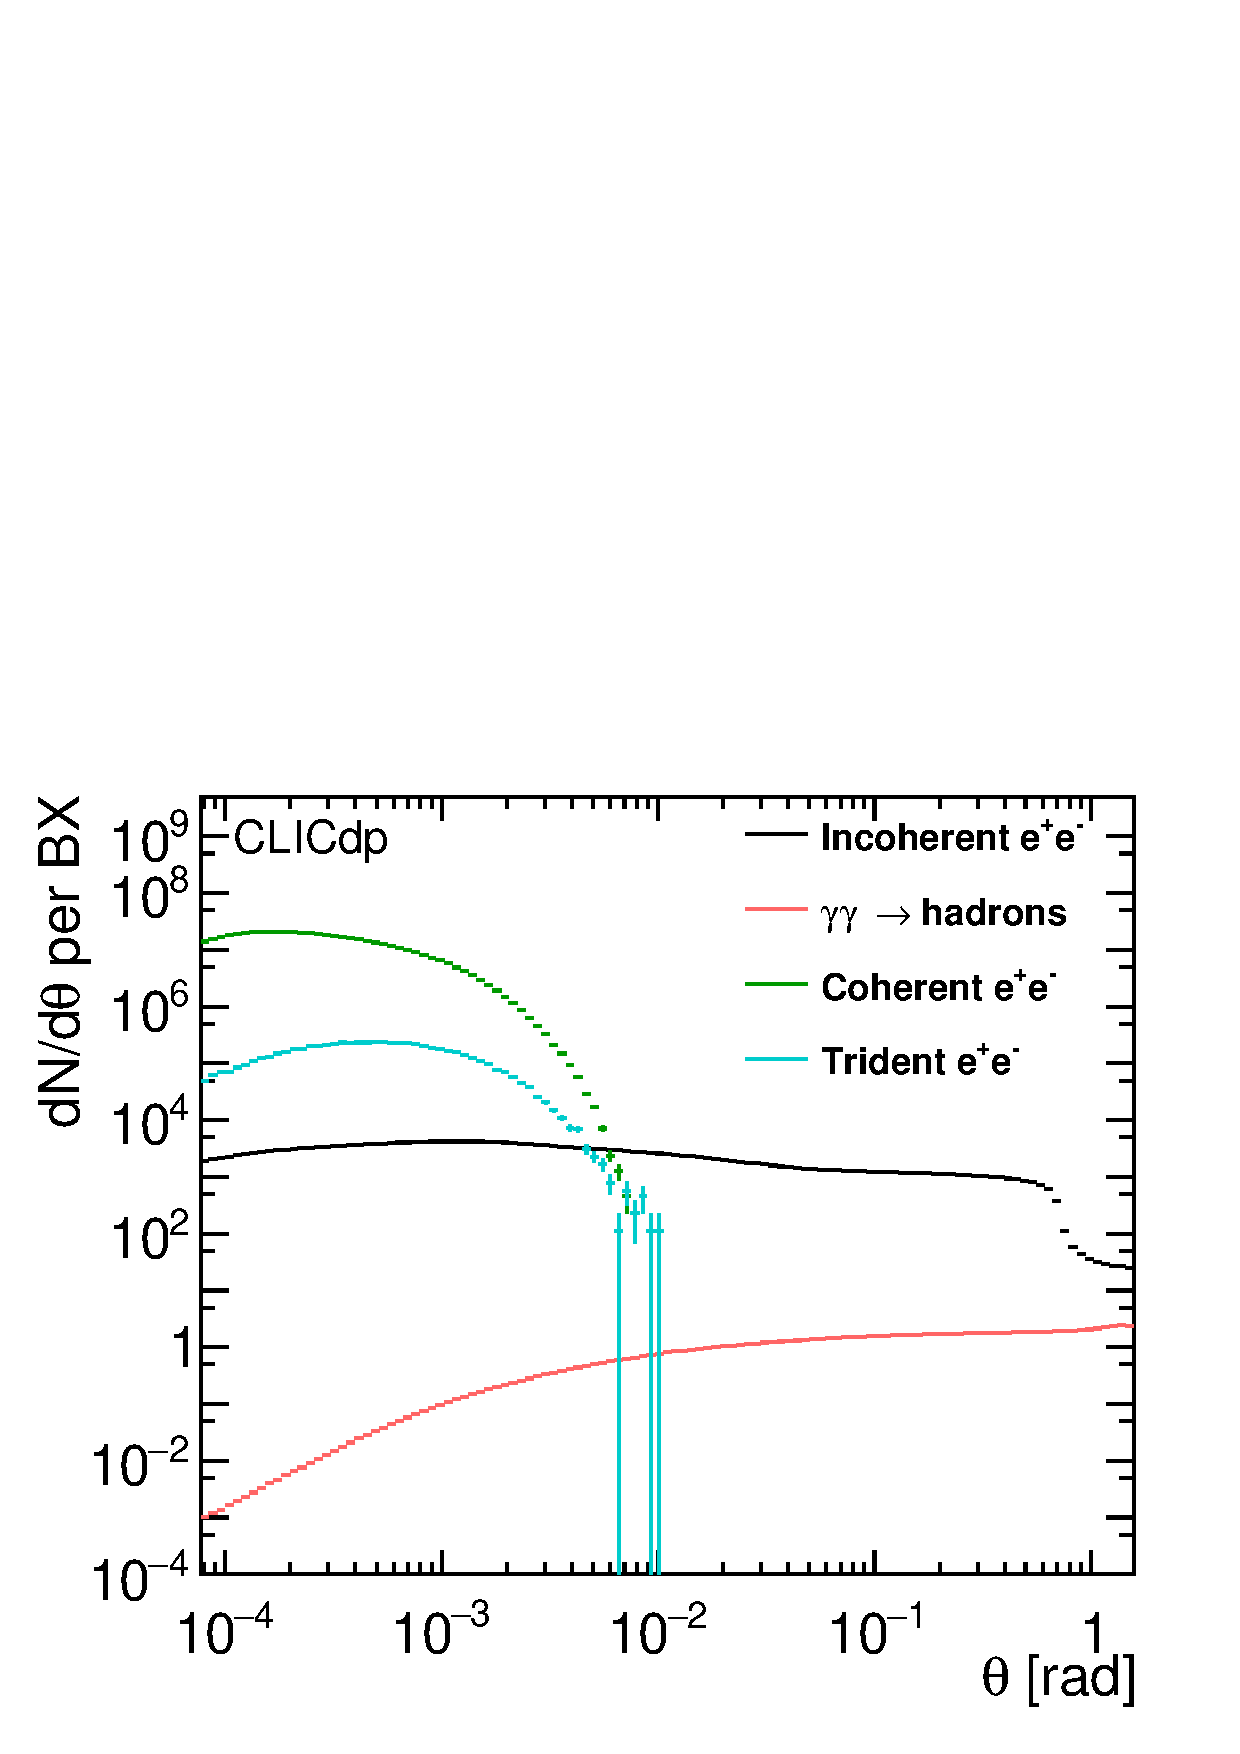
\includegraphics[width=7.0cm]{backgrounds_theta_3tev_l6.pdf}};

    \node[inner sep=0pt] (tmp) at (\xRefPosOne-0.9,\yRefPosOne+0.6)
    {\tiny WORK IN PROGRESS};
    
\end{tikzpicture}
  
\end{frame}
%*****************************************************************************
\backupend

\end{document}

